\documentclass[12pt,a4paper]{report}

\usepackage[a4paper,margin=1in]{geometry}
\usepackage[T1]{fontenc}
\usepackage[utf8]{inputenc}
\usepackage{lmodern}
\usepackage{setspace}
\usepackage{graphicx}
\usepackage{float}
\usepackage{booktabs}
\usepackage{longtable}
\usepackage{array}
\usepackage{multirow}
\usepackage{caption}
\usepackage{subcaption}
\usepackage{amsmath}
\usepackage{hyperref}
\usepackage{xcolor}
\usepackage{pdflscape}
\usepackage{enumitem}
\usepackage{fancyhdr}

\newcolumntype{L}[1]{>{\raggedright\arraybackslash}p{#1}}
\newcolumntype{C}[1]{>{\centering\arraybackslash}p{#1}}

\hypersetup{
    colorlinks=true,
    linkcolor=blue!50!black,
    urlcolor=blue!50!black,
    citecolor=blue!50!black
}

\setstretch{1.2}
\setlength{\parskip}{6pt}
\setlength{\parindent}{0pt}
\pagestyle{plain}

\begin{document}

\begin{titlepage}
    \centering
    \vspace*{0.4cm}
    
\includegraphics[width=4.2cm]{images/logo.png}\\[0.5cm]
    {\Large \textbf{Somaiya Vidyavihar University}}\\[0.2cm]
    {\Large \textbf{K. J. Somaiya College of Engineering}}\\[1.2cm]

    {\Large \textbf{PM$_{2.5}$ Estimation over Delhi-NCR}}\\[0.3cm]
    {\large Final Term Project Report}\\[0.8cm]

    {\normalsize Submitted in partial fulfillment of requirements}\\
    {\normalsize for the Degree of}\\[0.2cm]
    {\large \textbf{Bachelor of Technology}}\\
    {\normalsize (Artificial Intelligence and Data Science)}\\[1cm]

    {\normalsize By}\\[0.2cm]
    \begin{tabular}{ll}
        \textbf{Rajdeep Pandey} & Roll No: 16014223064 \\
        \textbf{Vruddhi Mule} & Roll No: 16014223099 \\
        \textbf{Sagar Jadhav} & Roll No: 16014223070 \\
        \textbf{Sohom Mallick} & Roll No: 16014223083 \\
    \end{tabular}\\[0.8cm]

    {\normalsize Group Number: 38}\\[0.8cm]
    {\normalsize Under the Guidance of}\\[0.2cm]
    {\large \textbf{Dr. Suchitra Patil}}\\[1.2cm]

    {\normalsize Third Year, AIDS}\\[0.2cm]
    {\normalsize 2023--27}\\[1.4cm]

    {\normalsize Mumbai - 400077}
\end{titlepage}

\begin{titlepage}
    \centering
    {\Large \textbf{Somaiya Vidyavihar University}}\\[0.2cm]
    {\Large \textbf{K. J. Somaiya College of Engineering}}\\[1.2cm]
    {\Large \textbf{Certificate}}\\[1cm]

    This is to certify that the project report entitled \textbf{PM$_{2.5}$ Estimation over Delhi-NCR} submitted by \textbf{Rajdeep Pandey, Vruddhi Mule, Sagar Jadhav, and Sohom Mallick} at the end of Semester VI of Third Year B. Tech is a bona fide record of the work carried out by the group under our guidance, in partial fulfillment of the requirements for the degree of \textbf{Bachelor of Technology} in \textbf{Artificial Intelligence and Data Science} of Somaiya Vidyavihar University.\\[2cm]

    \begin{tabular}{p{5cm}p{5cm}}
        \centering\rule{5cm}{0.4pt} & \centering\rule{5cm}{0.4pt} \\
        \centering Guide & \centering Head of the Department \\
    \end{tabular}\\[2cm]

    \begin{tabular}{p{5cm}}
        \centering\rule{5cm}{0.4pt} \\
        \centering Principal \\
    \end{tabular}

    \vfill
    Date: \rule{4cm}{0.4pt} \hfill Place: Mumbai-77
\end{titlepage}

\begin{titlepage}
    \centering
    {\Large \textbf{Somaiya Vidyavihar University}}\\[0.2cm]
    {\Large \textbf{K. J. Somaiya College of Engineering}}\\[1.2cm]
    {\Large \textbf{Declaration}}\\[1cm]

    We declare that this written report submission represents the work carried out by our group based on our understanding, implementation, and analysis with adequate acknowledgment of the original data sources, software packages, and references used in this project. We further declare that we have adhered to the principles of academic honesty and integrity, and that we have neither misrepresented nor fabricated any data, result, observation, or reference in this submission.\\[0.8cm]

    We understand that any violation of the above principles may lead to disciplinary action by the institute.\\[1.6cm]

    \begin{tabular}{p{7cm}p{5cm}}
        \rule{6cm}{0.4pt} & Roll No: 16014223064 \\
        Signature of Rajdeep Pandey & \\[0.6cm]
        \rule{6cm}{0.4pt} & Roll No: 16014223099 \\
        Signature of Vruddhi Mule & \\[0.6cm]
        \rule{6cm}{0.4pt} & Roll No: 16014223070 \\
        Signature of Sagar Jadhav & \\[0.6cm]
        \rule{6cm}{0.4pt} & Roll No: 16014223083 \\
        Signature of Sohom Mallick & \\
    \end{tabular}

    \vfill
    Date: \rule{4cm}{0.4pt} \hfill Place: Mumbai-77
\end{titlepage}

\begin{titlepage}
    \centering
    {\Large \textbf{Somaiya Vidyavihar University}}\\[0.2cm]
    {\Large \textbf{K. J. Somaiya College of Engineering}}\\[1.2cm]
    {\Large \textbf{Certificate of Approval of Examiners}}\\[1cm]

    We certify that this project report entitled \textbf{PM$_{2.5}$ Estimation over Delhi-NCR} is a bona fide record of project work carried out by \textbf{Rajdeep Pandey, Vruddhi Mule, Sagar Jadhav, and Sohom Mallick} during Semester VI of Third Year B. Tech.\\[0.8cm]

    This project work is submitted at the end of Semester VI in partial fulfillment of the requirements for the degree of \textbf{Bachelor of Technology} in \textbf{Artificial Intelligence and Data Science} of Somaiya Vidyavihar University.\\[2cm]

    \begin{tabular}{p{6cm}p{6cm}}
        \centering\rule{5cm}{0.4pt} & \centering\rule{5cm}{0.4pt} \\
        \centering Internal Examiner & \centering External / Expert Examiner \\
    \end{tabular}

    \vfill
    Date: \rule{4cm}{0.4pt} \hfill Place: Mumbai-77
\end{titlepage}

\pagenumbering{roman}

\chapter*{Abstract}
\addcontentsline{toc}{chapter}{Abstract}

This project addresses PM$_{2.5}$ estimation over Delhi-NCR using a reproducible multi-source environmental data workflow and comparative machine learning analysis. During the semester, pollutant observations, meteorological variables, and geospatial context features were collected from authentic external data sources and organized into a unified station-date modeling framework. The collected data were processed into a structured master table with temporal, seasonal, and lag-based features suitable for machine learning.

The work was carried out in two phases. The mid-semester phase focused on building the full data collection and preprocessing pipeline, implementing an XGBoost baseline, and creating a dashboard for presentation. The final-term phase extended this work by implementing an Artificial Neural Network (ANN), tuning the ANN configuration, and comparing ANN against XGBoost using the same engineered features and the same chronological holdout split. The final faculty-facing evaluation was designed to preserve fairness in model comparison by keeping the feature space, training protocol, and test horizon constant across both models.

The current dataset contains 29,240 daily station-date PM$_{2.5}$ rows across 40 harmonized station IDs spanning the period from 1 January 2023 to 31 December 2024. The final test comparison contains 5,880 rows covering the holdout period from 7 August 2024 to 31 December 2024. Final test metrics show that ANN slightly outperforms XGBoost on the current saved split, with ANN achieving RMSE 21.96, MAE 17.06, and R$^2$ 0.9295, compared with XGBoost RMSE 22.36, MAE 17.21, and R$^2$ 0.9269.

The final contribution of the semester is therefore not only a predictive model, but a complete project pipeline including collected data integration, preprocessing, feature engineering, comparative model evaluation, and a presentation-oriented dashboard for faculty review.

\tableofcontents
\listoffigures
\listoftables
\clearpage

\chapter*{Nomenclature}
\addcontentsline{toc}{chapter}{Nomenclature}
\begin{longtable}{L{2.5cm}L{11cm}}
\toprule
\textbf{Symbol / Term} & \textbf{Meaning} \\
\midrule
PM$_{2.5}$ & Fine particulate matter with aerodynamic diameter less than or equal to 2.5 micrometers \\
ERA5-Land & Land-surface reanalysis meteorological dataset used for atmospheric variables \\
ANN & Artificial Neural Network \\
MAE & Mean Absolute Error \\
RMSE & Root Mean Squared Error \\
R$^2$ & Coefficient of determination \\
MAPE & Mean Absolute Percentage Error \\
sMAPE & Symmetric Mean Absolute Percentage Error \\
\texttt{pm25\_lag1} & One-day lag of PM$_{2.5}$ for the same station \\
\texttt{pm25\_roll3\_mean} & Rolling 3-day average PM$_{2.5}$ value \\
\texttt{month\_sin}, \texttt{month\_cos} & Cyclic calendar encodings for seasonal learning \\
\bottomrule
\end{longtable}

\clearpage
\pagenumbering{arabic}

\chapter{Introduction}

\section{Problem Definition}
Air pollution forecasting is an important problem in environmental intelligence, particularly in a city such as Delhi-NCR where PM$_{2.5}$ levels vary significantly over time and across localities. PM$_{2.5}$ is affected by weather conditions, emissions, land-use intensity, atmospheric stability, and seasonal transitions. Because of this, reliable estimation requires more than raw pollutant observations. It requires a structured framework that integrates pollutant measurements with weather and contextual features.

The core problem addressed in this work is therefore the estimation of daily PM$_{2.5}$ concentration over a harmonized station framework in Delhi-NCR using collected multi-source environmental data and machine learning.

\section{Motivation}
The motivation for this project arises from three main observations:

\begin{itemize}[leftmargin=1.3cm]
    \item PM$_{2.5}$ behavior in Delhi-NCR is severe, dynamic, and highly seasonal.
    \item Traditional manual interpretation of environmental observations does not scale well across time and station networks.
    \item Machine learning offers a way to combine pollutant history, seasonal signals, and meteorology into a predictive system.
\end{itemize}

From an academic point of view, the project also provides a realistic applied-data-science problem that involves source integration, preprocessing, feature engineering, modeling, and evaluation rather than only isolated algorithm training.

\section{Scope}
The scope of the project during this semester includes:

\begin{itemize}[leftmargin=1.3cm]
    \item collection of PM$_{2.5}$ data from OpenAQ,
    \item collection of ERA5-Land weather variables,
    \item inclusion of elevation and urban-context variables,
    \item formation of a station-date master table,
    \item XGBoost baseline development,
    \item ANN development for final-term comparison,
    \item final model comparison through a faculty-oriented dashboard.
\end{itemize}

The project does not attempt to produce a production-grade citywide map service or a satellite-driven spatial surface. Its scope in the current semester remains station-level predictive modeling with fair comparison of two machine learning approaches.

\section{Salient Contributions}
The main contributions of the project are:

\begin{enumerate}[leftmargin=1.3cm]
    \item construction of a collected multi-source environmental dataset for Delhi-NCR,
    \item development of a reproducible preprocessing and feature-engineering workflow,
    \item implementation of an XGBoost baseline,
    \item implementation and tuning of an ANN model,
    \item fair ANN vs XGBoost evaluation on the same split,
    \item faculty-facing reporting and dashboard integration.
\end{enumerate}

\section{Organization of the Report}
This report is organized to follow the expected final project format. Chapter 2 summarizes the literature and domain background. Chapter 3 describes the software project management plan and semester execution structure. Chapter 4 presents the software requirements specification. Chapter 5 explains the dataset in detail. Chapter 6 presents system design and methodology. Chapter 7 explains model implementation. Chapter 8 presents results and comparison. Chapter 9 discusses the dashboard and presentation layer. Chapter 10 concludes the report and identifies future scope.

\chapter{Literature Survey}

Environmental PM$_{2.5}$ estimation has been studied using statistical models, tree-based machine learning methods, and neural approaches. Traditional linear and regression-based methods are often insufficient when pollutant behavior is nonlinear and affected by interacting seasonal and meteorological variables. Tree-based ensemble methods such as gradient boosting are widely used in structured environmental datasets because they handle nonlinear interactions and mixed feature types effectively. On the other hand, neural networks are useful when there is sufficient structure and scale for learning more flexible nonlinear mappings.

In urban air-quality forecasting, the most important factors repeatedly discussed in the literature are:

\begin{itemize}[leftmargin=1.3cm]
    \item pollutant persistence and lagged dependence,
    \item weather variables such as temperature, precipitation, and wind,
    \item seasonal periodicity,
    \item spatial heterogeneity and local context.
\end{itemize}

The present project aligns with this understanding. Instead of training a model directly on raw PM$_{2.5}$ alone, the workflow integrates pollutant history, seasonality, and meteorological data. The final-term comparison between XGBoost and ANN also follows a standard literature expectation: tree-based models are strong baselines for tabular data, while neural networks can provide improvement if properly tuned.

\chapter{Software Project Management Plan}

\section{Introduction}
The project was managed in two connected phases across the semester. The first phase established the baseline data and modeling workflow. The second phase extended the work into final-term comparative evaluation and formal documentation.

\subsection{Project Overview}
The project objective was to build a complete PM$_{2.5}$ estimation workflow for Delhi-NCR using collected environmental data and machine learning. The project was designed to produce not only numerical results but also reusable artifacts such as dataset bundles, master tables, prediction outputs, and a dashboard.

\subsection{Project Deliverables}
The semester deliverables are:

\begin{itemize}[leftmargin=1.3cm]
    \item collected dataset bundle in \path{pm25_delhi_bundle/},
    \item merged master table in \path{model_outputs/delhi_pm25_master.csv},
    \item XGBoost and ANN comparison artifacts,
    \item feature-importance outputs,
    \item faculty-oriented Streamlit dashboard,
    \item final report and presentation materials.
\end{itemize}

\section{Project Organization}

\subsection{Software Process Model}
The practical process followed an iterative workflow:

\begin{enumerate}[leftmargin=1.3cm]
    \item identify sources and collect baseline data,
    \item preprocess and validate the data,
    \item engineer features,
    \item train a baseline model,
    \item evaluate, diagnose, and improve,
    \item add a second model for fair comparison,
    \item refine reporting and presentation.
\end{enumerate}

This process was incremental rather than purely linear. Midterm work generated a usable baseline, and final-term work improved the modeling and presentation layers.

\subsection{Roles and Responsibilities}
The group worked under a shared project structure. The responsibilities can be understood in broad form as:

\begin{itemize}[leftmargin=1.3cm]
    \item data collection and integration activities,
    \item model training and evaluation,
    \item dashboard and report refinement,
    \item presentation and documentation preparation.
\end{itemize}

Although the final report is submitted jointly, the complete output reflects collaborative implementation and iterative project development across the semester.

\subsection{Tools and Techniques}
The major tools and techniques used include:

\begin{itemize}[leftmargin=1.3cm]
    \item Python for data processing and model implementation,
    \item Pandas and NumPy for tabular analysis,
    \item XGBoost for boosted-tree modeling,
    \item scikit-learn for ANN and preprocessing,
    \item Streamlit for dashboard presentation,
    \item LaTeX for final documentation.
\end{itemize}

\section{Project Management Plan}

\subsection{Tasks}

\subsubsection{Description}
The semester tasks were organized around data, models, and presentation. Initial tasks focused on collection and harmonization. Mid-phase tasks focused on feature engineering and the XGBoost baseline. Final-phase tasks focused on ANN, fair model comparison, and refinement of the reporting interface.

\subsubsection{Deliverables and Milestones}
The main milestones were:

\begin{itemize}[leftmargin=1.3cm]
    \item completion of collected dataset bundle,
    \item preparation of the master table,
    \item successful XGBoost baseline at midterm,
    \item implementation of ANN in the final term,
    \item generation of a clean ANN vs XGBoost metrics export,
    \item completion of final report and final presentation package.
\end{itemize}

\subsubsection{Resources Needed}
The project required:

\begin{itemize}[leftmargin=1.3cm]
    \item internet-accessible APIs and data sources at collection time,
    \item Python environment with machine learning libraries,
    \item notebook and scripting environment,
    \item visualization and report-generation tools.
\end{itemize}

\subsubsection{Dependencies and Constraints}
The main dependencies were source availability, API access, and consistency of geospatial joins. Key constraints included:

\begin{itemize}[leftmargin=1.3cm]
    \item API reliability and authentication restrictions,
    \item quality of static context variables in the saved workspace,
    \item time available for tuning multiple model families,
    \item need to preserve a fair and defensible evaluation split.
\end{itemize}

\subsubsection{Risk and Contingencies}
The main risks during the semester were:

\begin{itemize}[leftmargin=1.3cm]
    \item sparse or unstable source coverage,
    \item noisy or inconsistent values across sources,
    \item model instability in ANN tuning,
    \item misleading presentation artifacts from poorly designed dashboards.
\end{itemize}

The contingency responses included repair utilities, stricter comparison exports, and simplification of the dashboard into a presentation-only view.

\subsection{Time Table}
The project timeline can be summarized as:

\begin{itemize}[leftmargin=1.3cm]
    \item early semester: data pipeline and bundle creation,
    \item mid semester: preprocessing and XGBoost baseline,
    \item late semester: ANN implementation and tuning,
    \item final stage: comparative evaluation, dashboard refinement, report, and presentation.
\end{itemize}

\chapter{Software Requirements Specification}

\section{Introduction}
The software requirements of the project are driven by the need to collect, process, model, and present environmental data in a reproducible manner. The software layer must therefore support both offline analysis and faculty-facing reporting.

\subsection{Product Overview}
The project product consists of:

\begin{itemize}[leftmargin=1.3cm]
    \item a data-collection notebook,
    \item a model-training notebook,
    \item model-comparison export scripts,
    \item a faculty-facing dashboard,
    \item report and presentation assets.
\end{itemize}

\section{Specific Requirements}

\subsection{External Interface Requirements}
The project interacts with the following external interfaces:

\begin{itemize}[leftmargin=1.3cm]
    \item OpenAQ API for PM$_{2.5}$ observations,
    \item CDS/ERA5-Land interface for weather data,
    \item geospatial data interfaces for elevation and urban context,
    \item Streamlit UI for final model presentation.
\end{itemize}

\subsection{Functional Requirements}
The implemented software must:

\begin{itemize}[leftmargin=1.3cm]
    \item ingest collected data files,
    \item create a harmonized station-date modeling table,
    \item compute lag and rolling features,
    \item train XGBoost and ANN,
    \item evaluate both models on the same test split,
    \item export metrics and predictions,
    \item present final results visually.
\end{itemize}

\subsection{Non-Functional Requirements}
Important non-functional expectations are:

\begin{itemize}[leftmargin=1.3cm]
    \item reproducibility of the workflow,
    \item interpretability of outputs,
    \item fair comparison methodology,
    \item clean and presentation-appropriate visualization.
\end{itemize}

\chapter{Dataset Collection and Description}

\section{Authentic External Data Sources}
The environmental variables used in this project were collected from authentic external sources rather than manually fabricated records. The major sources are summarized in Table~\ref{tab:sources}.

\begin{table}[H]
\centering
\caption{Primary external data sources used in the project}
\label{tab:sources}
\begin{tabular}{L{3.2cm}L{4.1cm}L{6.2cm}}
\toprule
\textbf{Data Source} & \textbf{Platform} & \textbf{Purpose in Project} \\
\midrule
PM$_{2.5}$ observations & OpenAQ API & Daily PM$_{2.5}$ values used as the target after station-date aggregation \\
Meteorology & ERA5-Land via CDS API & Temperature and precipitation context variables \\
Elevation & SRTM / terrain source & Static geographic feature for each station coordinate \\
Urban context & OSM / OSMnx features & Building- and road-context information around station coordinates \\
\bottomrule
\end{tabular}
\end{table}

\begin{figure}[H]
    \centering
    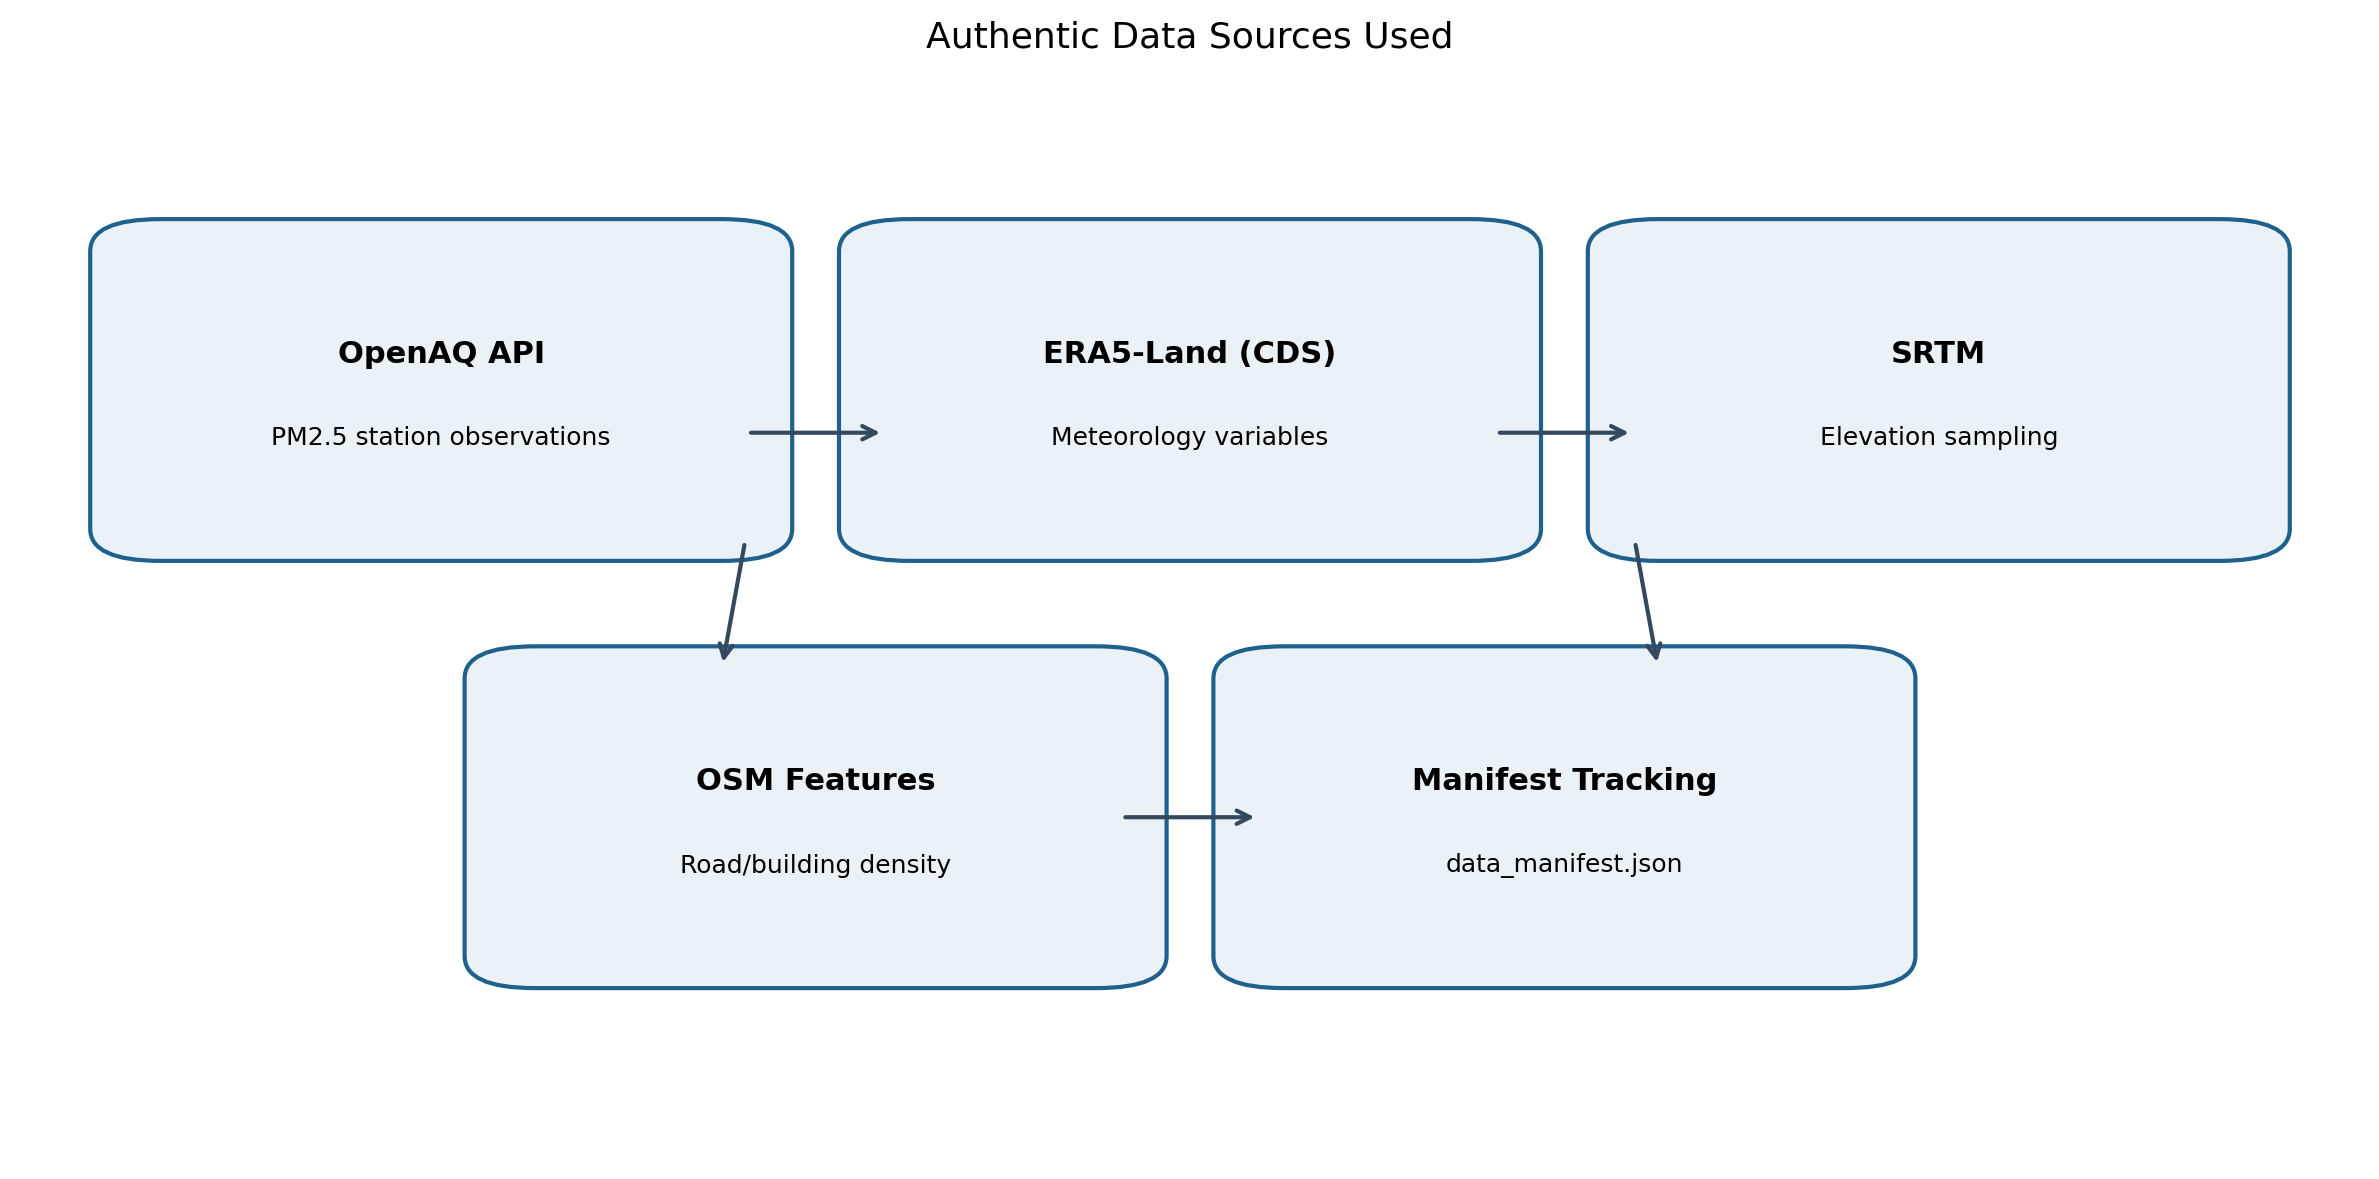
\includegraphics[width=0.88\textwidth]{images/slide05_data_sources_infographic.png}
    \caption{Overview of the external data sources used in the project}
\end{figure}

\subsection{Project Station Framework}
For source harmonization, a fixed project station framework was used over the Delhi region. This framework contains 40 station identifiers with latitude and longitude coordinates. These project station IDs serve as the common spatial reference used to merge PM$_{2.5}$ observations, meteorological variables, and static contextual attributes.

The role of this framework should be stated carefully: the environmental data themselves were collected from external sources, while the project station IDs were used as harmonized indexing keys for merging source outputs into a consistent station-date table.

\subsection{Collection Workflow}
The data-building pipeline is implemented in \path{01_build_download_dataset.ipynb}. The major operations are:

\begin{enumerate}[leftmargin=1.3cm]
    \item define station coordinates across the Delhi region,
    \item collect PM$_{2.5}$ observations,
    \item collect ERA5-Land meteorological variables,
    \item extract elevation values,
    \item compute urban-context features,
    \item package the collected and processed outputs.
\end{enumerate}

\begin{figure}[H]
    \centering
    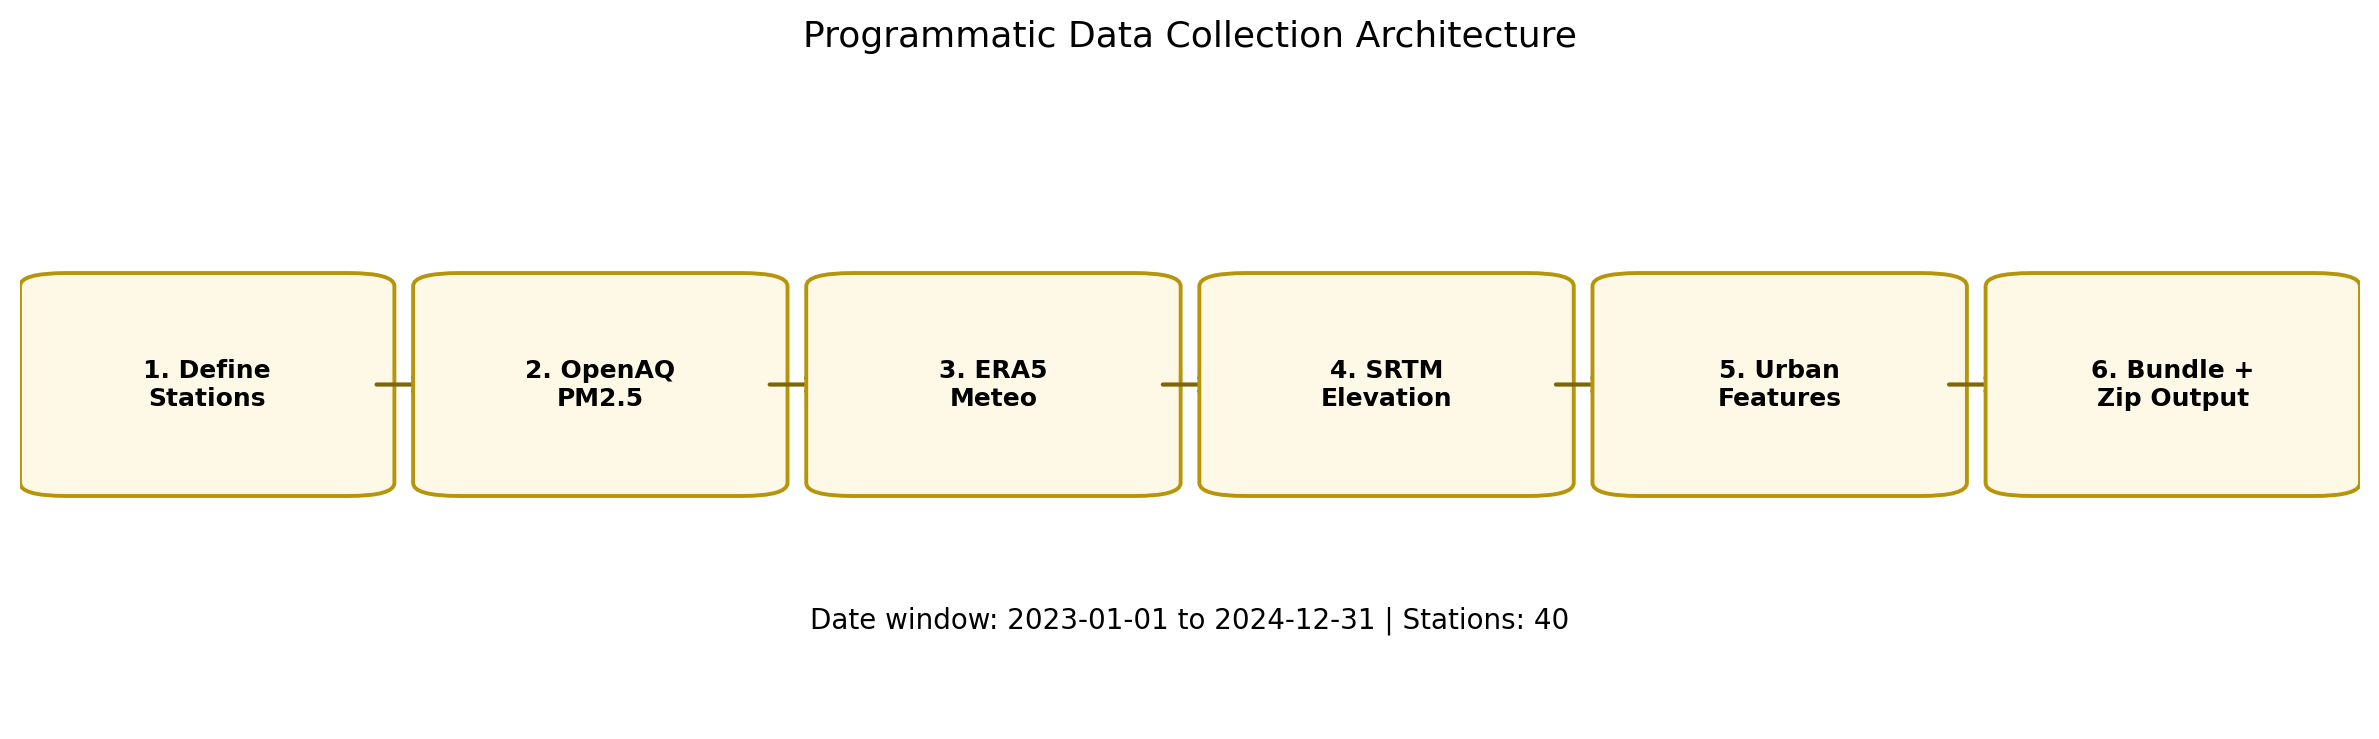
\includegraphics[width=0.90\textwidth]{images/slide06_collection_pipeline.png}
    \caption{High-level collection and packaging pipeline}
\end{figure}

\section{Dataset Inventory}
The current working bundle and modeling outputs contain the files listed in Table~\ref{tab:inventory}. These files are the primary evidence base for the final-term report.

\begingroup
\footnotesize
\setlength{\LTleft}{0pt}
\setlength{\LTright}{0pt}
\begin{longtable}{L{6.5cm}C{1.4cm}C{1.5cm}L{4.0cm}}
\caption{Inventory of major dataset and output files}\label{tab:inventory}\\
\toprule
\textbf{File} & \textbf{Rows} & \textbf{Stations} & \textbf{Description} \\
\midrule
\endfirsthead
\toprule
\textbf{File} & \textbf{Rows} & \textbf{Stations} & \textbf{Description} \\
\midrule
\endhead
\path{pm25_delhi_bundle/stations_urban.csv} & 40 & 40 & Station coordinates and urban-context attributes \\
\path{pm25_delhi_bundle/stations_elevation.csv} & 40 & 40 & Elevation values for station coordinates \\
\path{pm25_delhi_bundle/openaq_pm25.csv} & 29,240 & 40 & Daily PM$_{2.5}$ target table \\
\path{pm25_delhi_bundle/era5_meteo.csv} & 29,240 & 40 & Daily meteorological context table \\
\path{model_outputs/delhi_pm25_master.csv} & 29,240 & 40 & Final merged and engineered station-date modeling table \\
\path{model_outputs/model_predictions_compare.csv} & 5,880 & 40 & Test-period predictions and errors for ANN vs XGBoost \\
\path{model_outputs/model_comparison_metrics.csv} & 2 & -- & Final model comparison metrics \\
\path{model_outputs/feature_importance.csv} & 64 & -- & Saved XGBoost feature-importance output \\
\bottomrule
\end{longtable}
\endgroup

\section{Temporal Coverage}
The current PM$_{2.5}$ and meteorological data cover the period from \textbf{2023-01-01} to \textbf{2024-12-31}. Thus the dataset spans two full calendar years. The final faculty-facing evaluation file contains only the holdout period used for testing, namely \textbf{2024-08-07} to \textbf{2024-12-31}.

\section{Detailed Attribute Description}

\subsection{\texttt{stations\_urban.csv}}
\begin{longtable}{L{3cm}L{2cm}L{8.6cm}}
\caption{Attribute description for \texttt{stations\_urban.csv}}\\
\toprule
\textbf{Attribute} & \textbf{Type} & \textbf{Description} \\
\midrule
\endfirsthead
\toprule
\textbf{Attribute} & \textbf{Type} & \textbf{Description} \\
\midrule
\endhead
\texttt{lat} & numeric & Latitude of the project station coordinate \\
\texttt{lon} & numeric & Longitude of the project station coordinate \\
\texttt{source} & text & Source label used for the station framework \\
\texttt{station\_id} & text & Project station identifier used for source harmonization \\
\texttt{building\_density} & numeric & Urban-context building-density feature around the station coordinate \\
\texttt{road\_density} & numeric & Urban-context road-density feature around the station coordinate \\
\bottomrule
\end{longtable}

\subsection{\texttt{stations\_elevation.csv}}
\begin{longtable}{L{3cm}L{2cm}L{8.6cm}}
\caption{Attribute description for \texttt{stations\_elevation.csv}}\\
\toprule
\textbf{Attribute} & \textbf{Type} & \textbf{Description} \\
\midrule
\endfirsthead
\toprule
\textbf{Attribute} & \textbf{Type} & \textbf{Description} \\
\midrule
\endhead
\texttt{lat} & numeric & Latitude of station coordinate \\
\texttt{lon} & numeric & Longitude of station coordinate \\
\texttt{source} & text & Source label associated with the station framework \\
\texttt{station\_id} & text & Station identifier \\
\texttt{elevation} & numeric & Elevation value sampled from terrain source \\
\bottomrule
\end{longtable}

\subsection{\texttt{openaq\_pm25.csv}}
\begin{longtable}{L{3cm}L{2cm}L{8.6cm}}
\caption{Attribute description for \texttt{openaq\_pm25.csv}}\\
\toprule
\textbf{Attribute} & \textbf{Type} & \textbf{Description} \\
\midrule
\endfirsthead
\toprule
\textbf{Attribute} & \textbf{Type} & \textbf{Description} \\
\midrule
\endhead
\texttt{station\_id} & text & Harmonized project station ID \\
\texttt{date} & date & Observation date after daily aggregation \\
\texttt{pm25} & numeric & Daily mean PM$_{2.5}$ concentration in $\mu g/m^3$ \\
\bottomrule
\end{longtable}

\subsection{\texttt{era5\_meteo.csv}}
\begin{longtable}{L{3cm}L{2cm}L{8.6cm}}
\caption{Attribute description for \texttt{era5\_meteo.csv}}\\
\toprule
\textbf{Attribute} & \textbf{Type} & \textbf{Description} \\
\midrule
\endfirsthead
\toprule
\textbf{Attribute} & \textbf{Type} & \textbf{Description} \\
\midrule
\endhead
\texttt{valid\_time} & datetime & Time associated with the ERA5 record \\
\texttt{t2m} & numeric & 2-meter air temperature \\
\texttt{tp} & numeric & Total precipitation \\
\texttt{number} & numeric & Source export field \\
\texttt{latitude} & numeric & Latitude of extracted ERA5 point \\
\texttt{longitude} & numeric & Longitude of extracted ERA5 point \\
\texttt{expver} & numeric & ERA5 export/version field \\
\texttt{station\_id} & text & Project station ID used for joining \\
\bottomrule
\end{longtable}

\subsection{\texttt{delhi\_pm25\_master.csv}}
\begin{longtable}{L{3.2cm}L{2cm}L{8.4cm}}
\caption{Attribute description for \texttt{delhi\_pm25\_master.csv}}\\
\toprule
\textbf{Attribute} & \textbf{Type} & \textbf{Description} \\
\midrule
\endfirsthead
\toprule
\textbf{Attribute} & \textbf{Type} & \textbf{Description} \\
\midrule
\endhead
\texttt{station\_id} & text & Harmonized station identifier \\
\texttt{date} & date & Daily timestamp for the row \\
\texttt{pm25} & numeric & Daily PM$_{2.5}$ concentration \\
\texttt{log\_pm25} & numeric & Log-transformed target using $\log(1+\text{PM}_{2.5})$ \\
\texttt{pm25\_lag1} & numeric & Previous-day PM$_{2.5}$ value for the same station \\
\texttt{pm25\_lag2} & numeric & 2-day lag PM$_{2.5}$ value \\
\texttt{pm25\_lag3} & numeric & 3-day lag PM$_{2.5}$ value \\
\texttt{pm25\_lag7} & numeric & 7-day lag PM$_{2.5}$ value \\
\texttt{pm25\_roll3\_mean} & numeric & Rolling 3-day mean PM$_{2.5}$ \\
\texttt{pm25\_roll7\_mean} & numeric & Rolling 7-day mean PM$_{2.5}$ \\
\texttt{pm25\_roll7\_std} & numeric & Rolling 7-day standard deviation \\
\texttt{month}, \texttt{dayofweek}, \texttt{dayofyear} & numeric & Calendar variables \\
\texttt{month\_sin}, \texttt{month\_cos} & numeric & Month cycle encodings \\
\texttt{dow\_sin}, \texttt{dow\_cos} & numeric & Day-of-week cycle encodings \\
\texttt{doy\_sin}, \texttt{doy\_cos} & numeric & Day-of-year cycle encodings \\
\texttt{temp\_2m}, \texttt{total\_precip} & numeric & Harmonized meteorological variables \\
\texttt{lat}, \texttt{lon} & numeric & Station coordinates \\
\texttt{building\_density}, \texttt{road\_density}, \texttt{elevation} & numeric & Static contextual features \\
\bottomrule
\end{longtable}

\section{Descriptive Statistics of PM$_{2.5}$}

\begin{table}[H]
\centering
\caption{Descriptive statistics of PM$_{2.5}$ values}
\begin{tabular}{lc}
\toprule
\textbf{Statistic} & \textbf{Value} \\
\midrule
Count & 29,240 \\
Mean & 118.48 \\
Median & 96.99 \\
Mode & 10.00 \\
Standard deviation & 71.75 \\
Minimum & 5.00 \\
25th percentile & 63.18 \\
75th percentile & 174.24 \\
Maximum & 308.52 \\
\bottomrule
\end{tabular}
\end{table}

The PM$_{2.5}$ distribution is right-skewed, with the mean higher than the median. This indicates that high-pollution episodes influence the average strongly, which is expected for Delhi-NCR during winter months.

\begin{figure}[H]
    \centering
    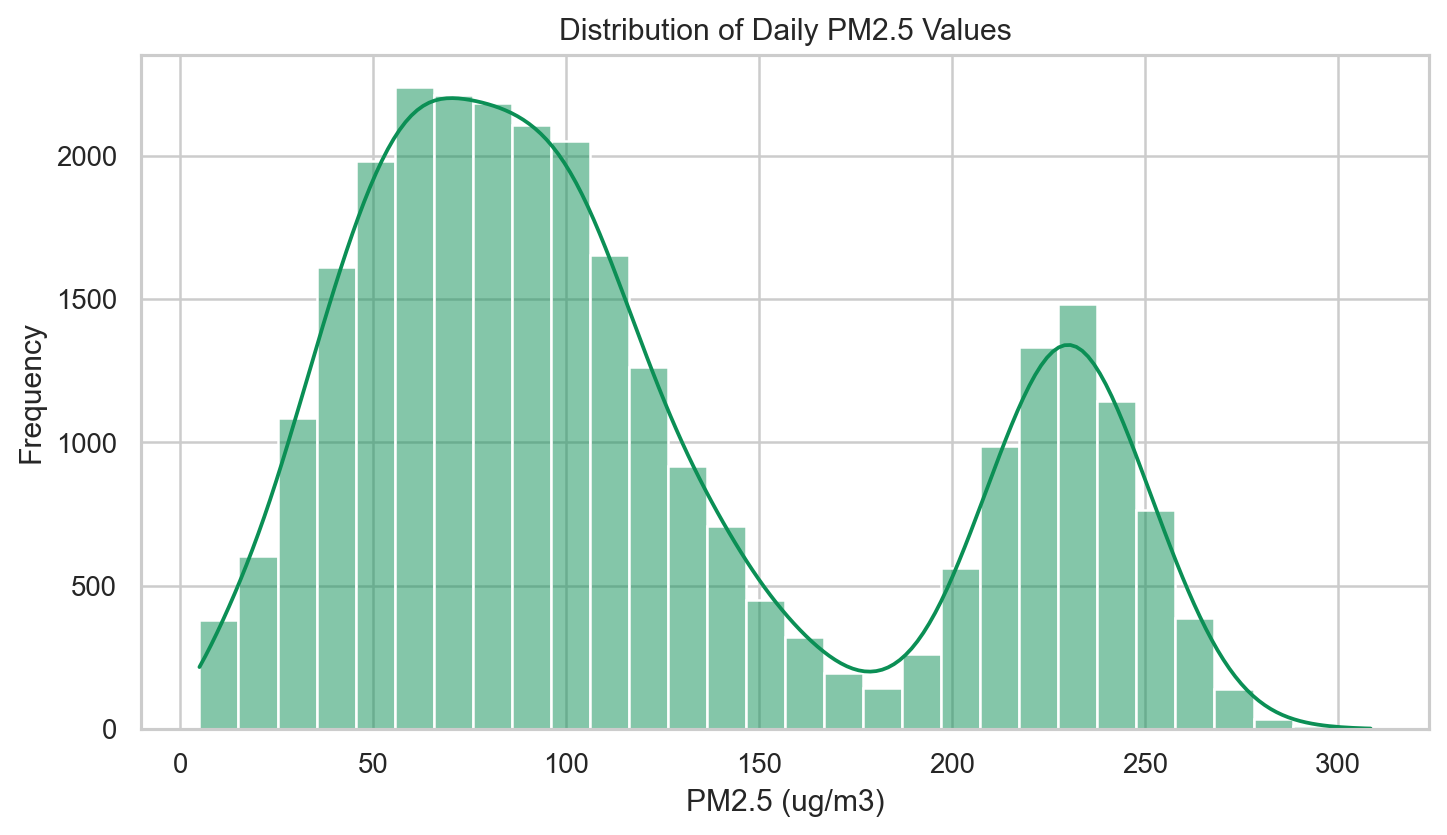
\includegraphics[width=0.82\textwidth]{figures/pm25_distribution.png}
    \caption{Distribution of daily PM$_{2.5}$ values}
\end{figure}

\section{Seasonal Characteristics}
The monthly pattern confirms strong seasonality. PM$_{2.5}$ is highest in January, November, and December, and lowest in July, August, and September.

\begin{table}[H]
\centering
\caption{Monthly PM$_{2.5}$ summary across 2023--2024}
\begin{tabular}{lrrrr}
\toprule
\textbf{Month} & \textbf{Mean} & \textbf{Median} & \textbf{Min} & \textbf{Max} \\
\midrule
January & 227.27 & 230.21 & 5.00 & 302.06 \\
February & 99.92 & 100.15 & 5.00 & 198.24 \\
March & 100.35 & 100.89 & 5.00 & 253.94 \\
April & 99.45 & 99.54 & 9.76 & 195.47 \\
May & 75.77 & 75.13 & 5.00 & 236.01 \\
June & 76.06 & 75.27 & 5.00 & 292.64 \\
July & 49.53 & 48.54 & 5.00 & 222.29 \\
August & 48.96 & 47.84 & 5.00 & 206.65 \\
September & 49.85 & 48.59 & 5.00 & 228.67 \\
October & 138.89 & 139.68 & 5.00 & 205.68 \\
November & 226.76 & 229.42 & 7.96 & 300.58 \\
December & 226.75 & 229.26 & 5.00 & 308.52 \\
\bottomrule
\end{tabular}
\end{table}

\begin{figure}[H]
    \centering
    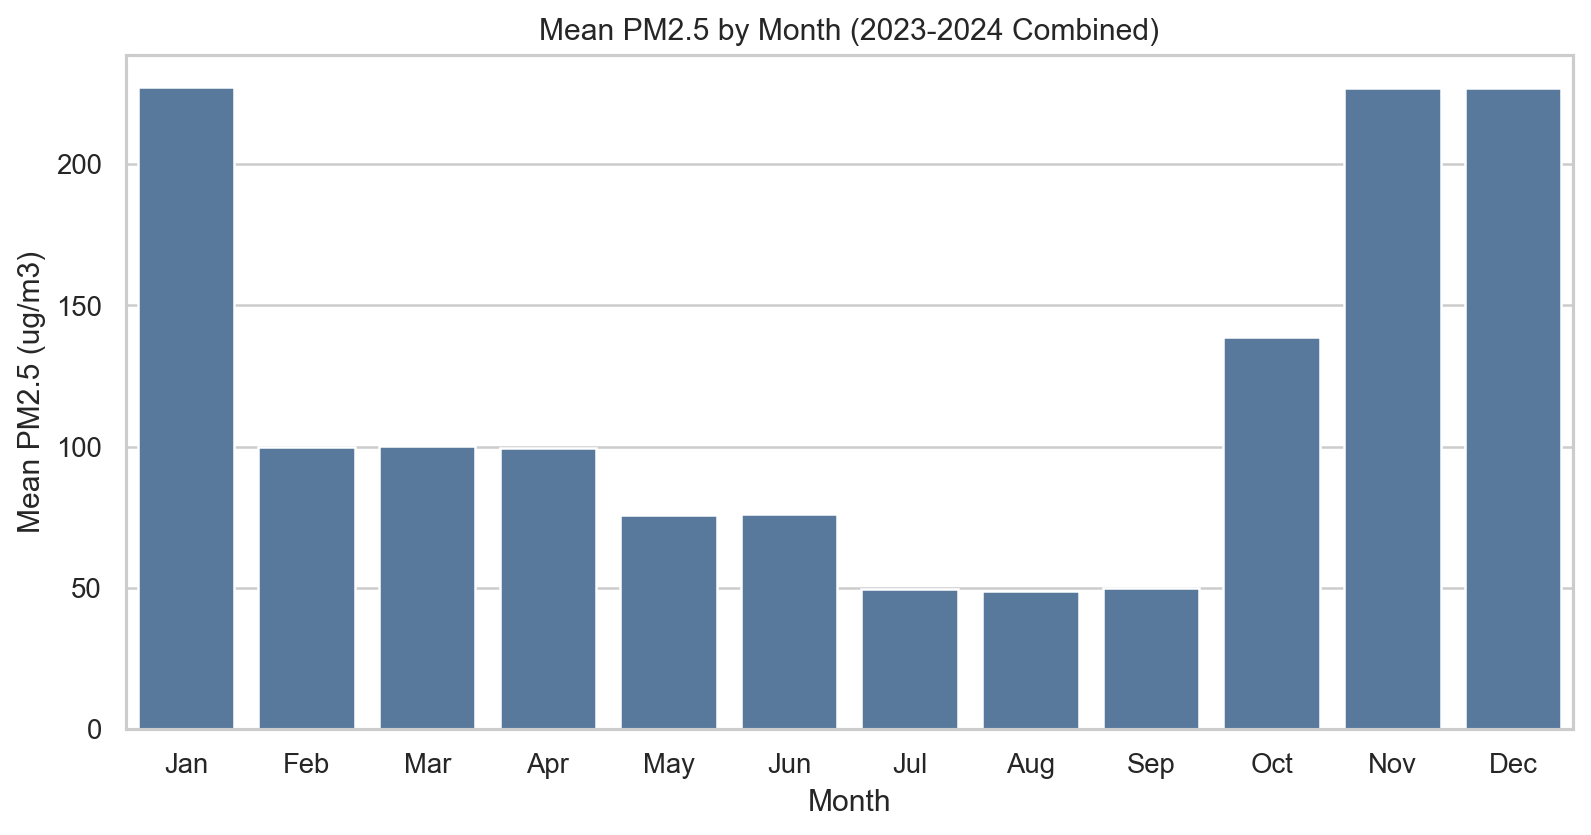
\includegraphics[width=0.84\textwidth]{figures/monthly_mean_pm25.png}
    \caption{Mean PM$_{2.5}$ by month}
\end{figure}

\section{Correlation and Missingness}
Correlation analysis indicates that recent PM$_{2.5}$ history is one of the strongest drivers of current PM$_{2.5}$ in the saved dataset. The strongest positive correlations are with rolling means and lag values. Temperature shows a strong negative relation, which is consistent with the seasonal structure of the data.

\begin{figure}[H]
    \centering
    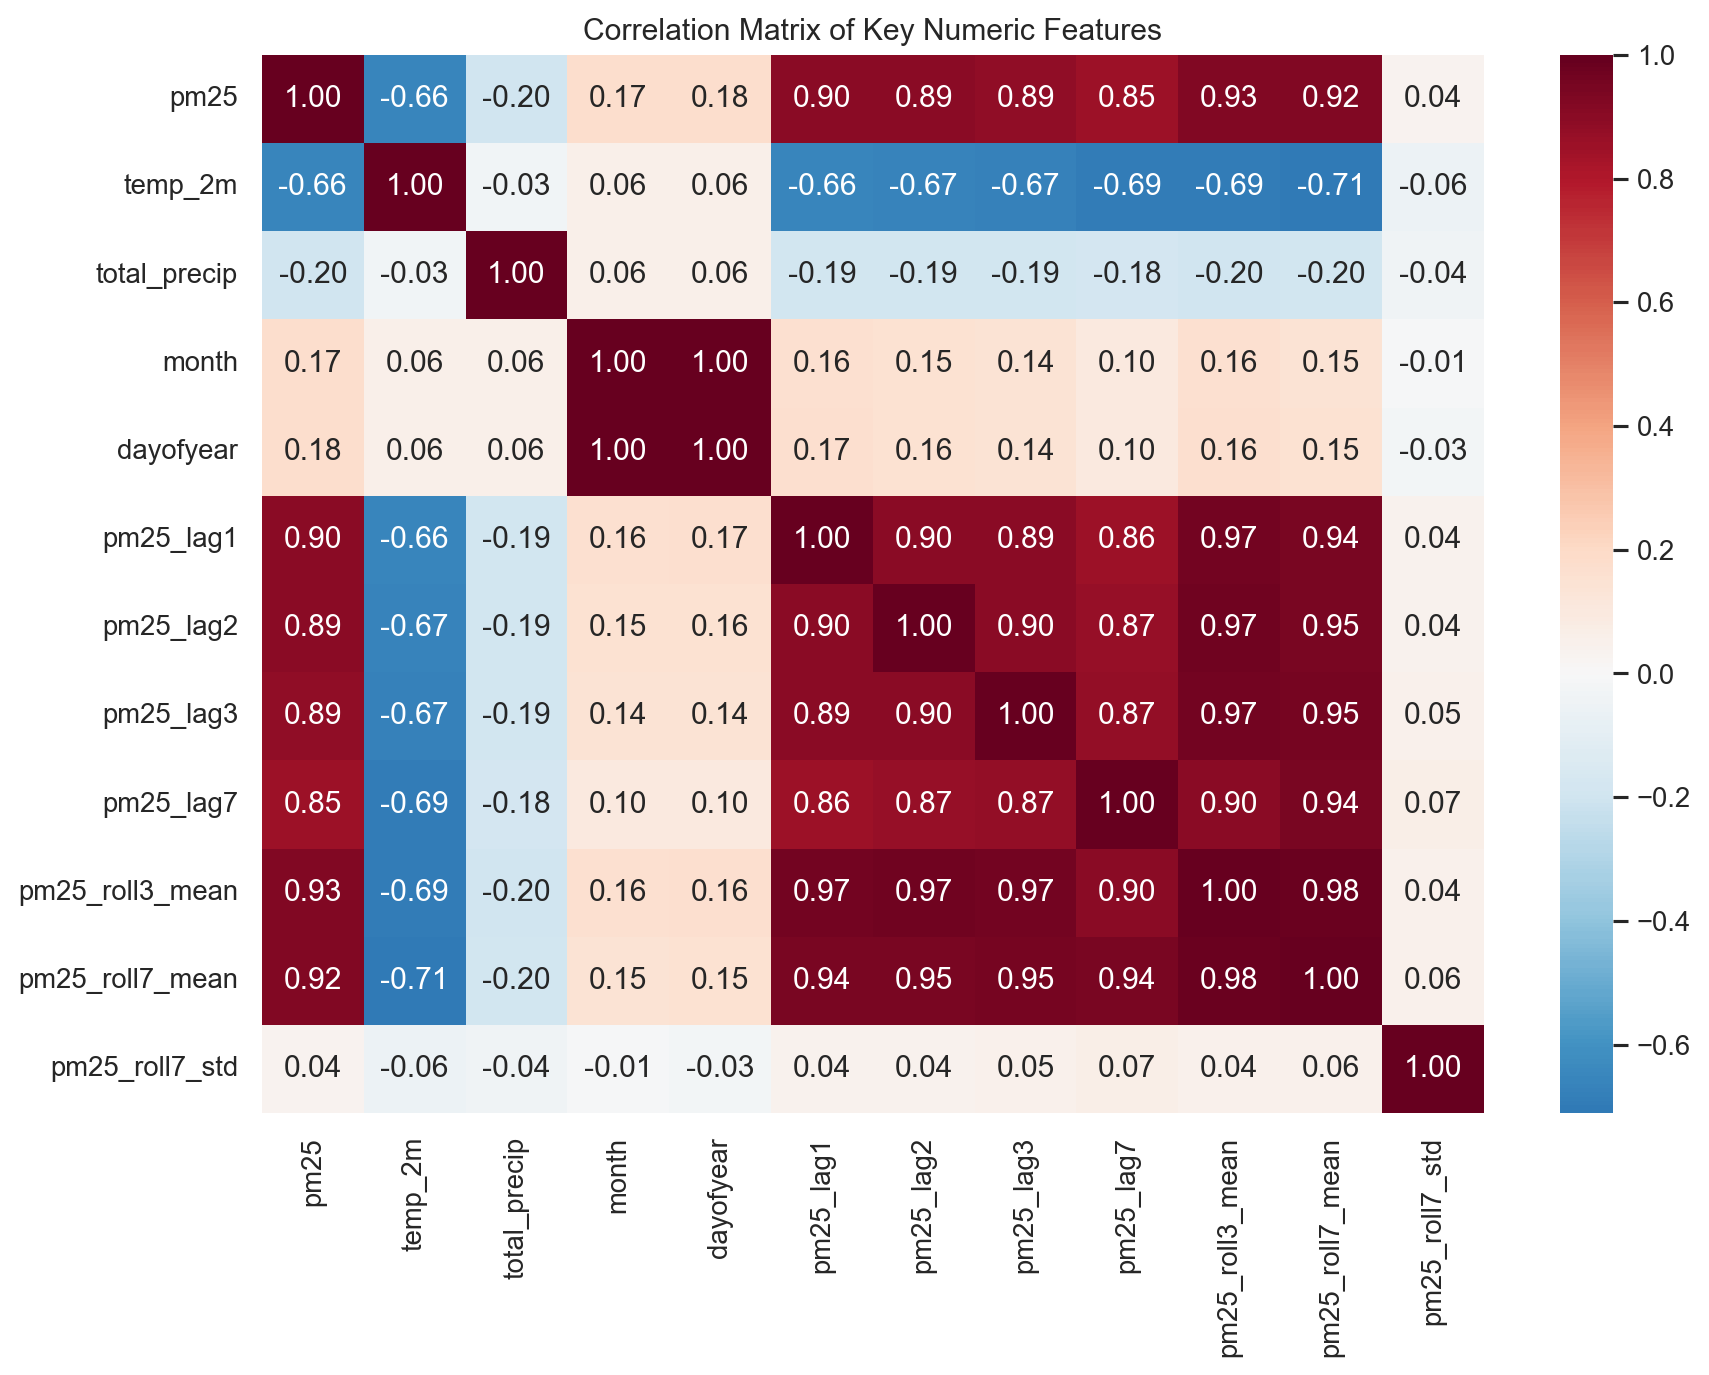
\includegraphics[width=0.92\textwidth]{figures/correlation_heatmap.png}
    \caption{Correlation matrix of key numeric variables}
\end{figure}

Lag and rolling features contain expected missing values at the beginning of each station sequence because those values cannot be computed until sufficient historical context exists.

\begin{figure}[H]
    \centering
    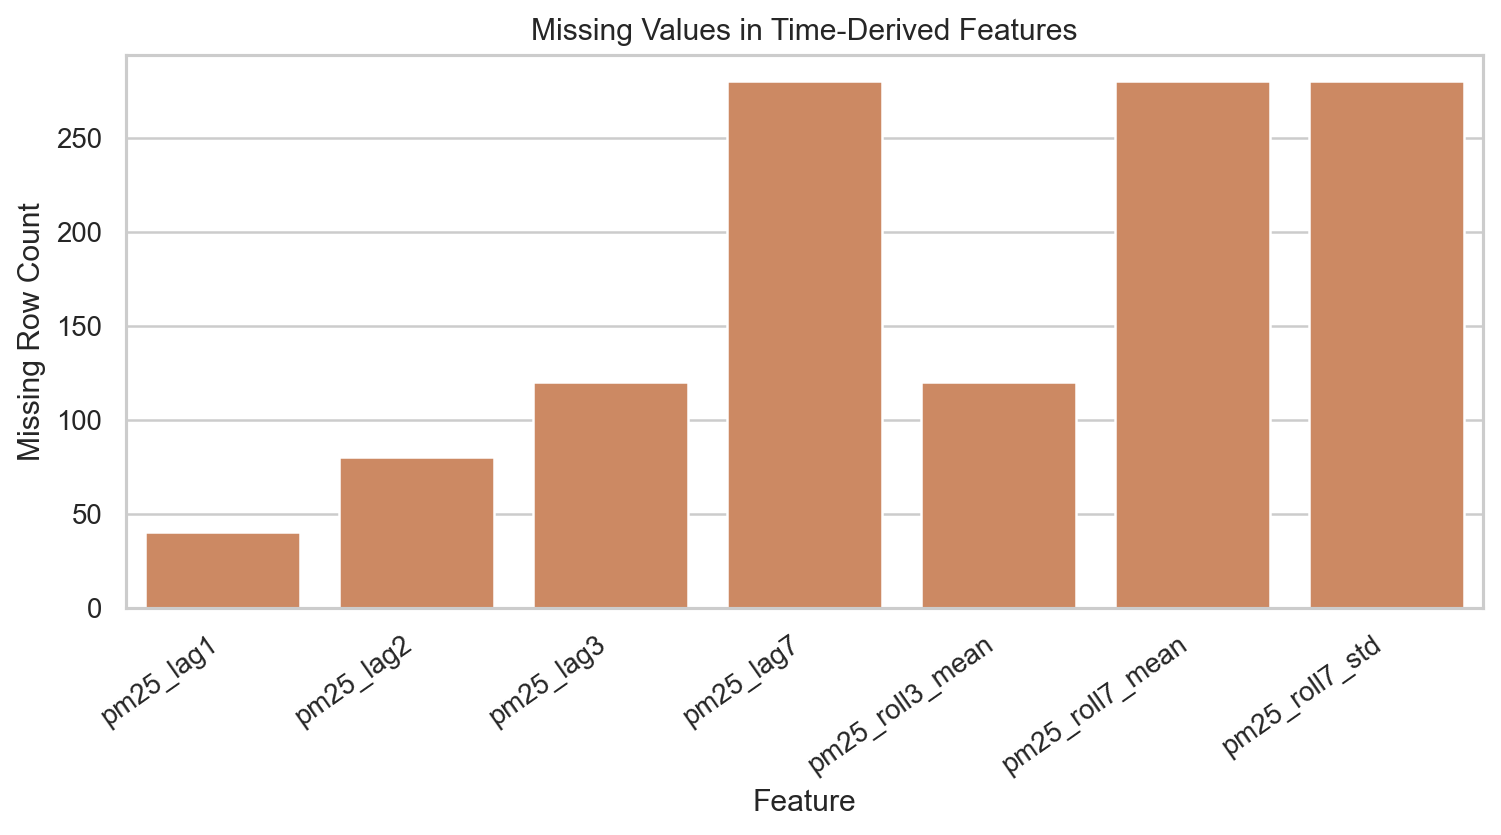
\includegraphics[width=0.82\textwidth]{figures/missing_values_lags.png}
    \caption{Missing values in lag and rolling features}
\end{figure}

\section{Important Caveats in the Saved Workspace}
The current saved workspace contains some caveats that must be acknowledged honestly:

\begin{itemize}[leftmargin=1.3cm]
    \item \texttt{building\_density} and \texttt{road\_density} are constant at zero in the current saved station-context file.
    \item \texttt{elevation} is constant at 216 in the current saved elevation file.
    \item \texttt{data\_manifest.json} does not match the current PM$_{2.5}$ file row count.
\end{itemize}

These issues do not invalidate the reported final ANN vs XGBoost comparison, but they are important for transparent reporting.

\chapter{System Design and Methodology}

\section{Overall Workflow}
The practical workflow of the project is:

\begin{enumerate}[leftmargin=1.3cm]
    \item collect and cache environmental source data,
    \item harmonize data into a station-date table,
    \item preprocess and validate numeric fields,
    \item generate temporal and lag-based features,
    \item train and evaluate models,
    \item save comparison artifacts,
    \item present outputs through the dashboard.
\end{enumerate}

\begin{figure}[H]
    \centering
    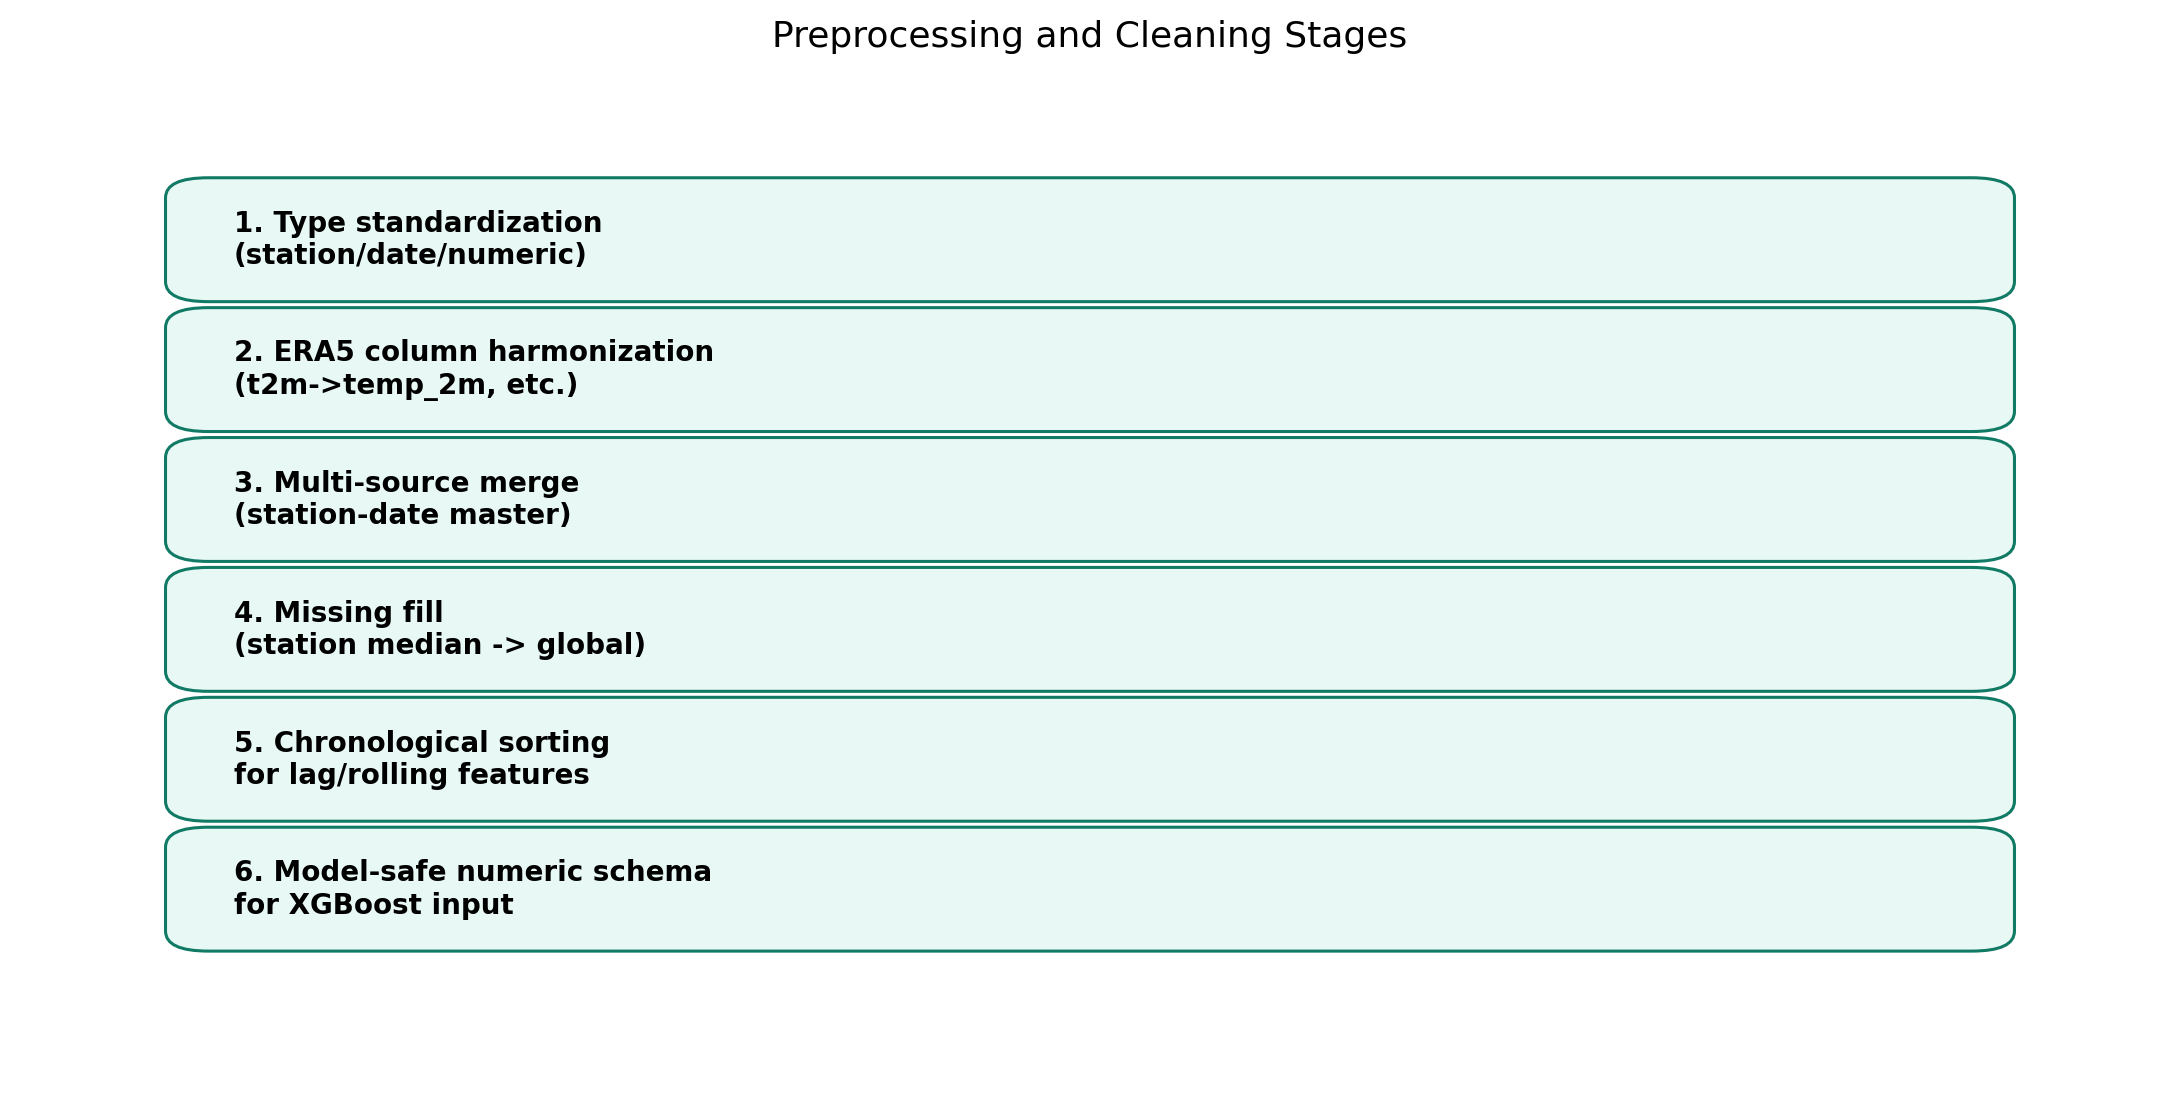
\includegraphics[width=0.85\textwidth]{images/slide08_preprocessing_pipeline.png}
    \caption{Preprocessing and feature-engineering pipeline}
\end{figure}

\section{Preprocessing and Harmonization}
The preprocessing logic is implemented mainly in \path{02_train_xgboost_model.ipynb}. The major operations are:

\begin{itemize}[leftmargin=1.3cm]
    \item parsing dates consistently,
    \item converting all numeric variables into machine-learning-safe numeric types,
    \item harmonizing ERA5 variable names,
    \item joining PM$_{2.5}$, meteorology, and static station attributes into one table,
    \item sorting rows chronologically within each station.
\end{itemize}

\section{Feature Engineering}
The feature engineering strategy was built around temporal dependence and seasonal structure.

\subsection{Temporal Features}
\begin{itemize}[leftmargin=1.3cm]
    \item month,
    \item day-of-week,
    \item day-of-year.
\end{itemize}

\subsection{Cyclic Encodings}
\begin{itemize}[leftmargin=1.3cm]
    \item \texttt{month\_sin}, \texttt{month\_cos},
    \item \texttt{dow\_sin}, \texttt{dow\_cos},
    \item \texttt{doy\_sin}, \texttt{doy\_cos}.
\end{itemize}

\subsection{Historical PM$_{2.5}$ Features}
\begin{itemize}[leftmargin=1.3cm]
    \item lags at 1, 2, 3, and 7 days,
    \item rolling 3-day mean,
    \item rolling 7-day mean,
    \item rolling 7-day standard deviation.
\end{itemize}

\subsection{Environmental and Spatial Features}
\begin{itemize}[leftmargin=1.3cm]
    \item temperature,
    \item precipitation,
    \item latitude and longitude,
    \item contextual static variables.
\end{itemize}

\section{Target Transformation}
The training target is transformed using:
\[
\texttt{log\_pm25} = \log(1 + \texttt{pm25})
\]
This improves numeric stability and reduces the dominance of the highest-pollution observations during optimization.

\chapter{Model Implementation}

\section{XGBoost Baseline}
The midterm baseline and continuing reference model is XGBoost regression. The final parameterization uses:

\begin{itemize}[leftmargin=1.3cm]
    \item \texttt{n\_estimators = 1200},
    \item \texttt{max\_depth = 6},
    \item \texttt{learning\_rate = 0.03},
    \item \texttt{subsample = 0.9},
    \item \texttt{colsample\_bytree = 0.9},
    \item \texttt{reg\_alpha = 0.1},
    \item \texttt{reg\_lambda = 2.0}.
\end{itemize}

XGBoost is suitable for this problem because it handles structured tabular data effectively and can model nonlinear interactions among lag features, weather variables, and calendar encodings.

\section{ANN Implementation}
The final-term ANN implementation is based on a multilayer perceptron and is now the clean comparison model used in the final dashboard.

The final ANN configuration uses:

\begin{itemize}[leftmargin=1.3cm]
    \item \texttt{MLPRegressor},
    \item hidden layers $(256, 128)$,
    \item ReLU activation,
    \item input scaling with \texttt{StandardScaler},
    \item target scaling through transformed target regression,
    \item early stopping,
    \item five-seed ensembling for stability.
\end{itemize}

The ANN was trained on exactly the same feature set and the same train/test partition as XGBoost. This preserves fairness in the final evaluation.

\section{Implementation Files}
The main files used during the semester are listed in Table~\ref{tab:implfiles}.

\begingroup
\footnotesize
\setlength{\LTleft}{0pt}
\setlength{\LTright}{0pt}
\begin{longtable}{L{5.3cm}L{8.3cm}}
\caption{Primary implementation files used during the semester}\label{tab:implfiles}\\
\toprule
\textbf{File} & \textbf{Role in Semester Work} \\
\midrule
\endfirsthead
\toprule
\textbf{File} & \textbf{Role in Semester Work} \\
\midrule
\endhead
\path{01_build_download_dataset.ipynb} & Data collection, harmonization, and dataset-bundle creation \\
\path{02_train_xgboost_model.ipynb} & Main training workflow, feature engineering, XGBoost baseline, and ANN comparison additions \\
\path{build_model_comparison.py} & Final-term model-only ANN vs XGBoost comparison export and metrics generation \\
\path{streamlit_app.py} & Faculty-facing comparison dashboard \\
\path{fix_dataset_temp.py} & Maintenance and repair utility for data issues \\
\bottomrule
\end{longtable}
\endgroup

\chapter{Evaluation Strategy and Results}

\section{Chronological Holdout Strategy}
The final comparison uses a per-station chronological split:

\begin{itemize}[leftmargin=1.3cm]
    \item first 80\% of each station timeline for training,
    \item last 20\% for testing.
\end{itemize}

This avoids leakage from future observations into training and preserves a realistic forecasting-style evaluation setup.

\begin{figure}[H]
    \centering
    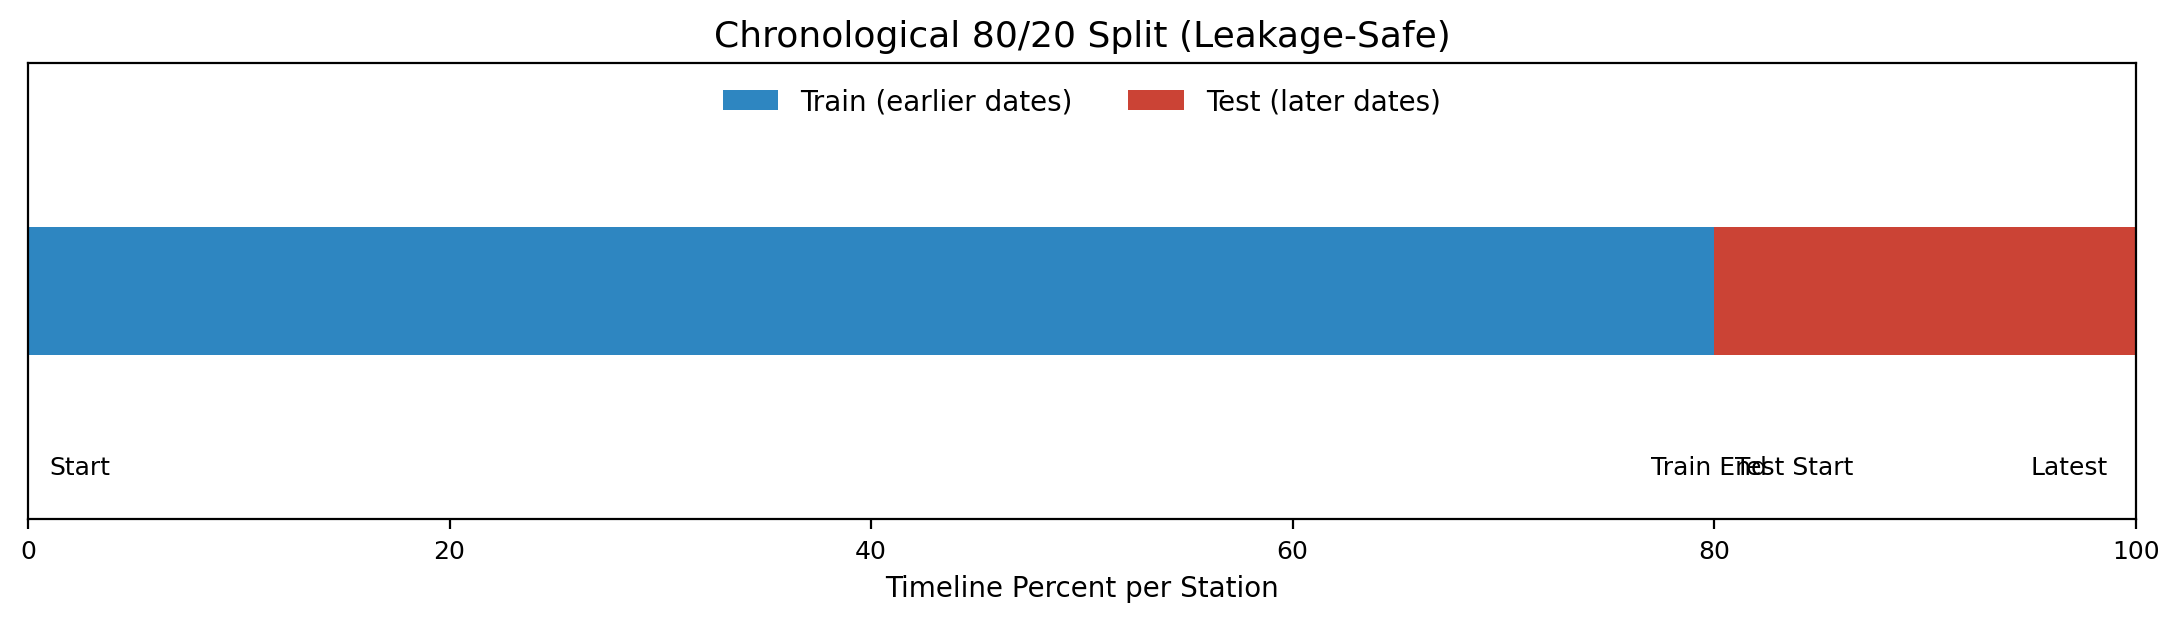
\includegraphics[width=0.78\textwidth]{images/slide10_chronological_split.png}
    \caption{Chronological train/test split}
\end{figure}

\section{Final Comparison Metrics}
The final model-only comparison intentionally includes only the two real models: ANN and XGBoost.

\begin{table}[H]
\centering
\caption{Final comparison metrics on the test set}
\begin{tabular}{lrrrrrrr}
\toprule
\textbf{Model} & \textbf{RMSE} & \textbf{MAE} & \textbf{R$^2$} & \textbf{Bias} & \textbf{sMAPE} & \textbf{MAPE} & \textbf{Rows} \\
\midrule
ANN & 21.96 & 17.06 & 0.9295 & -1.50 & 19.65 & 25.03 & 5880 \\
XGBoost & 22.36 & 17.21 & 0.9269 & -3.33 & 20.53 & 25.55 & 5880 \\
\bottomrule
\end{tabular}
\end{table}

The results show that ANN slightly outperforms XGBoost on the current saved split. The gain is modest but consistent across MAE, RMSE, and R$^2$.

\begin{figure}[H]
    \centering
    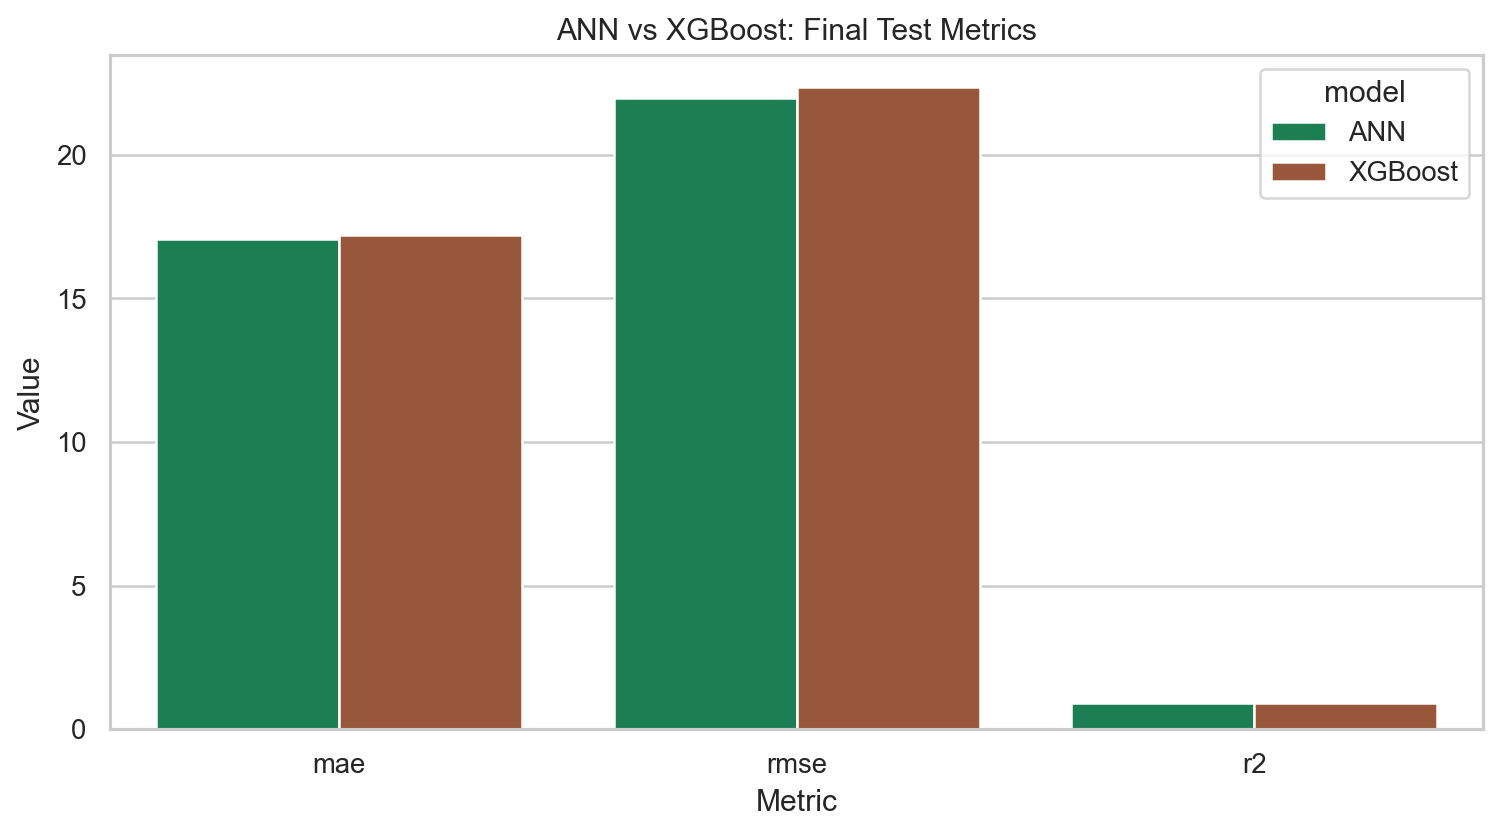
\includegraphics[width=0.76\textwidth]{figures/model_metrics_comparison.png}
    \caption{Final ANN vs XGBoost test metrics}
\end{figure}

\section{Feature-Level and Station-Level Interpretation}
The XGBoost feature-importance profile indicates that seasonality and recent PM$_{2.5}$ history dominate predictive signal in the saved workspace.

\begin{figure}[H]
    \centering
    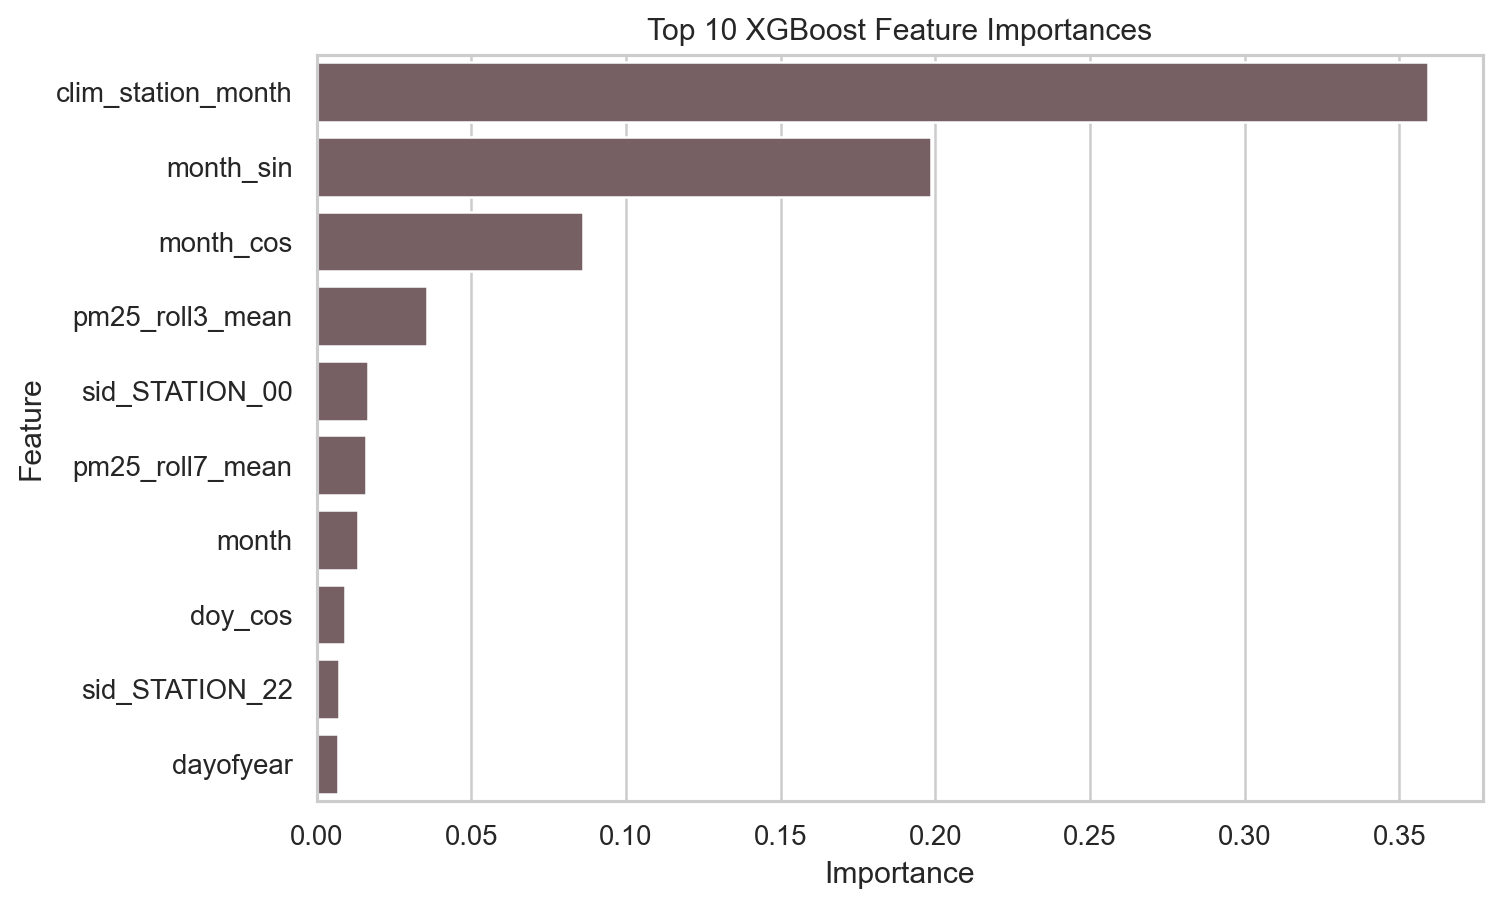
\includegraphics[width=0.76\textwidth]{figures/feature_importance_top10.png}
    \caption{Top ten XGBoost feature importances}
\end{figure}

Station-wise comparison shows that ANN improvement is not limited to a single isolated case. It achieves lower error than XGBoost on a meaningful subset of stations, although the overall difference remains small rather than dramatic.

\begin{figure}[H]
    \centering
    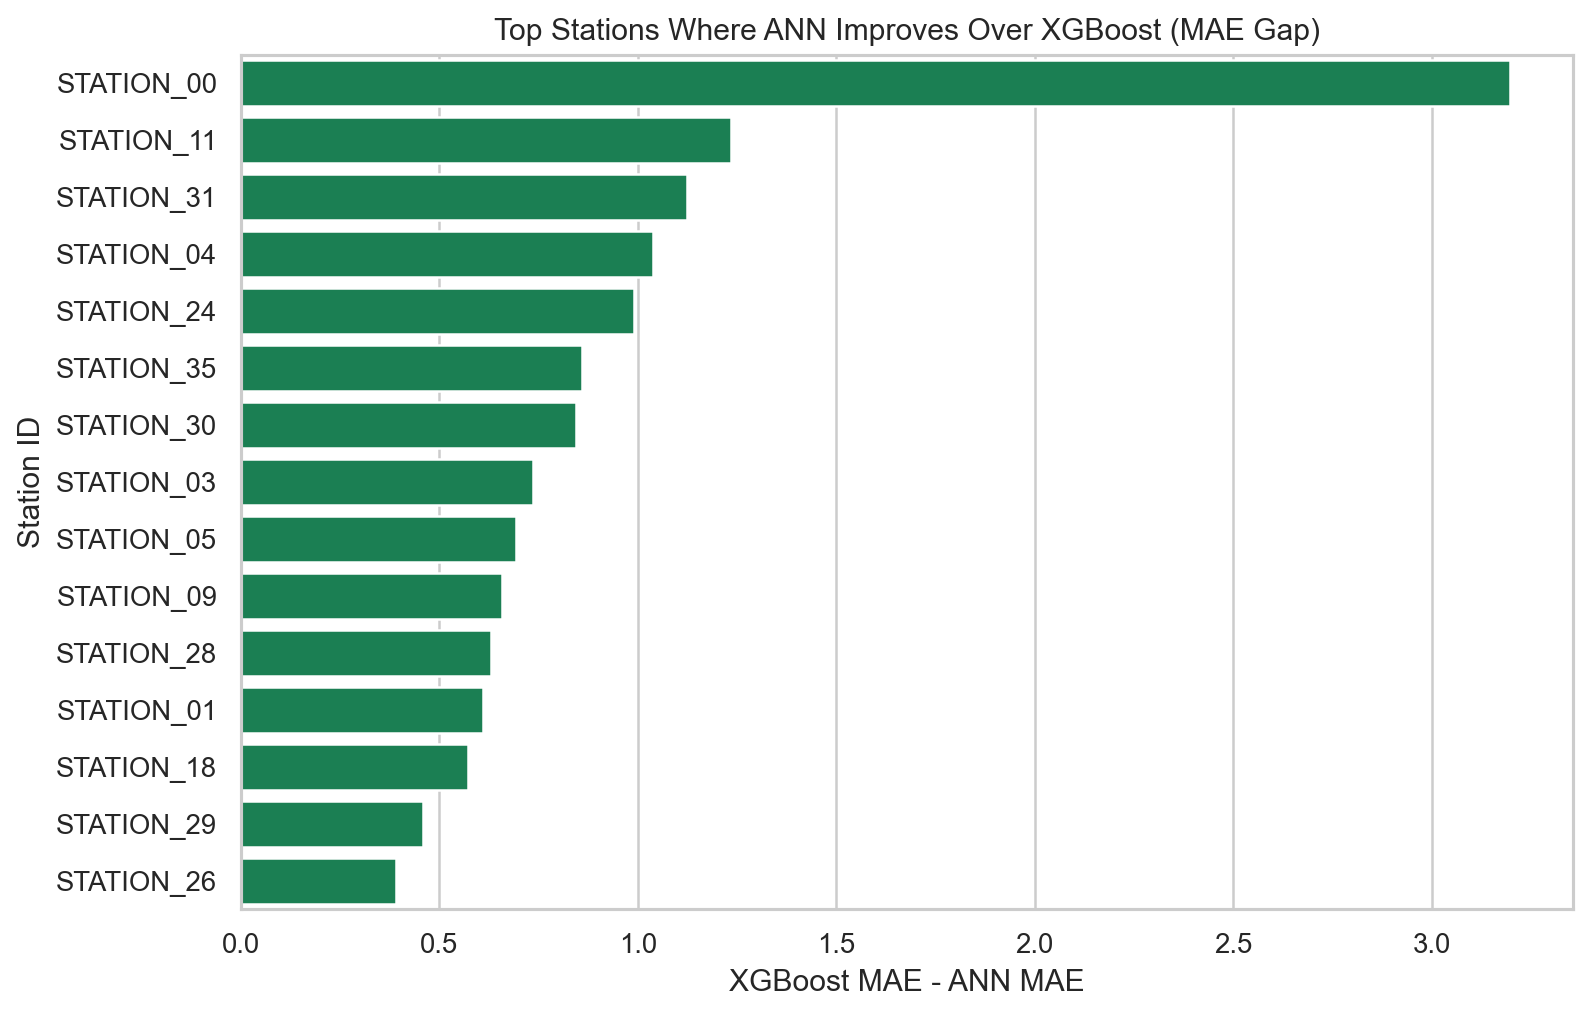
\includegraphics[width=0.80\textwidth]{figures/station_mae_gap.png}
    \caption{Stations where ANN improves over XGBoost}
\end{figure}

\section{Interpretation of the Results}
The closeness of ANN and XGBoost performance is itself meaningful. It indicates that:

\begin{itemize}[leftmargin=1.3cm]
    \item the current feature space already contains strong predictive structure,
    \item both models can learn the broader seasonal and lag-driven pattern,
    \item neither model completely captures all short-term spikes,
    \item ANN offers a real but modest improvement under the same evaluation protocol.
\end{itemize}

\chapter{Dashboard and Final Presentation Layer}

\section{Purpose of the Dashboard}
The Streamlit dashboard was refined into a faculty-facing comparison interface. Its purpose is to present only the information required for final evaluation rather than a cluttered development dashboard.

\section{Main Dashboard Components}
The final dashboard presents:

\begin{itemize}[leftmargin=1.3cm]
    \item a two-row metrics table for ANN and XGBoost,
    \item station-wise comparison,
    \item time-series behavior for a selected station and date window,
    \item parity visualization for both models.
\end{itemize}

\section{Why the Dashboard Was Simplified}
Earlier diagnostic views included baseline rows, multi-station line plots, and crowded debugging elements. These were removed because they do not improve faculty interpretation. The final version focuses only on the actual comparison question: how does ANN perform relative to XGBoost on the same test data?

\chapter{Conclusion and Future Scope}

\section{Conclusion}
This semester project established a complete PM$_{2.5}$ estimation workflow for Delhi-NCR, from collected source data to model comparison and faculty presentation. The major final-term addition was the implementation and tuning of ANN for direct comparison against the XGBoost baseline.

The final comparison shows that ANN is slightly better than XGBoost on the saved test split. Although the margin is not large, it is sufficient to conclude that the ANN is the stronger of the two implemented models under the current feature-engineering and evaluation framework.

\section{Future Scope}
Possible future extensions include:

\begin{itemize}[leftmargin=1.3cm]
    \item richer spatial-context features,
    \item improved preservation of source location metadata,
    \item sequence-aware or spatio-temporal neural models,
    \item better handling of short-term PM$_{2.5}$ spikes.
\end{itemize}

\chapter*{References}
\addcontentsline{toc}{chapter}{References}

\begin{enumerate}[leftmargin=1.0cm]
    \item OpenAQ. \textit{OpenAQ API Documentation and Platform Resources}. Available at: \url{https://docs.openaq.org/} and \url{https://explore.openaq.org/}.
    \item Copernicus Climate Data Store. \textit{ERA5-Land Reanalysis}. Available at: \url{https://cds.climate.copernicus.eu/}.
    \item OpenStreetMap Contributors. \textit{OpenStreetMap Data and Associated Tools}. Available at: \url{https://www.openstreetmap.org/}.
    \item Boeing, G. \textit{OSMnx: New Methods for Acquiring, Constructing, Analyzing, and Visualizing Complex Street Networks}. Available project/documentation resources at: \url{https://osmnx.readthedocs.io/}.
    \item NASA / SRTM Terrain Data Resources. \textit{Shuttle Radar Topography Mission Elevation Data}. Common access pathways include SRTM-derived raster sources used for terrain extraction.
    \item Chen, T. and Guestrin, C. (2016). \textit{XGBoost: A Scalable Tree Boosting System}. Proceedings of the 22nd ACM SIGKDD International Conference on Knowledge Discovery and Data Mining.
    \item Pedregosa, F. et al. (2011). \textit{Scikit-learn: Machine Learning in Python}. Journal of Machine Learning Research, 12, 2825--2830.
    \item Scikit-learn Developers. \textit{scikit-learn Documentation}. Available at: \url{https://scikit-learn.org/}.
    \item Streamlit. \textit{Streamlit Documentation}. Available at: \url{https://docs.streamlit.io/}.
    \item Hunter, J. D. (2007). \textit{Matplotlib: A 2D Graphics Environment}. Computing in Science and Engineering, 9(3), 90--95.
    \item Waskom, M. L. (2021). \textit{seaborn: statistical data visualization}. Journal of Open Source Software, 6(60), 3021.
\end{enumerate}

\appendix

\chapter{Selected Supporting Figures}

\begin{figure}[H]
    \centering
    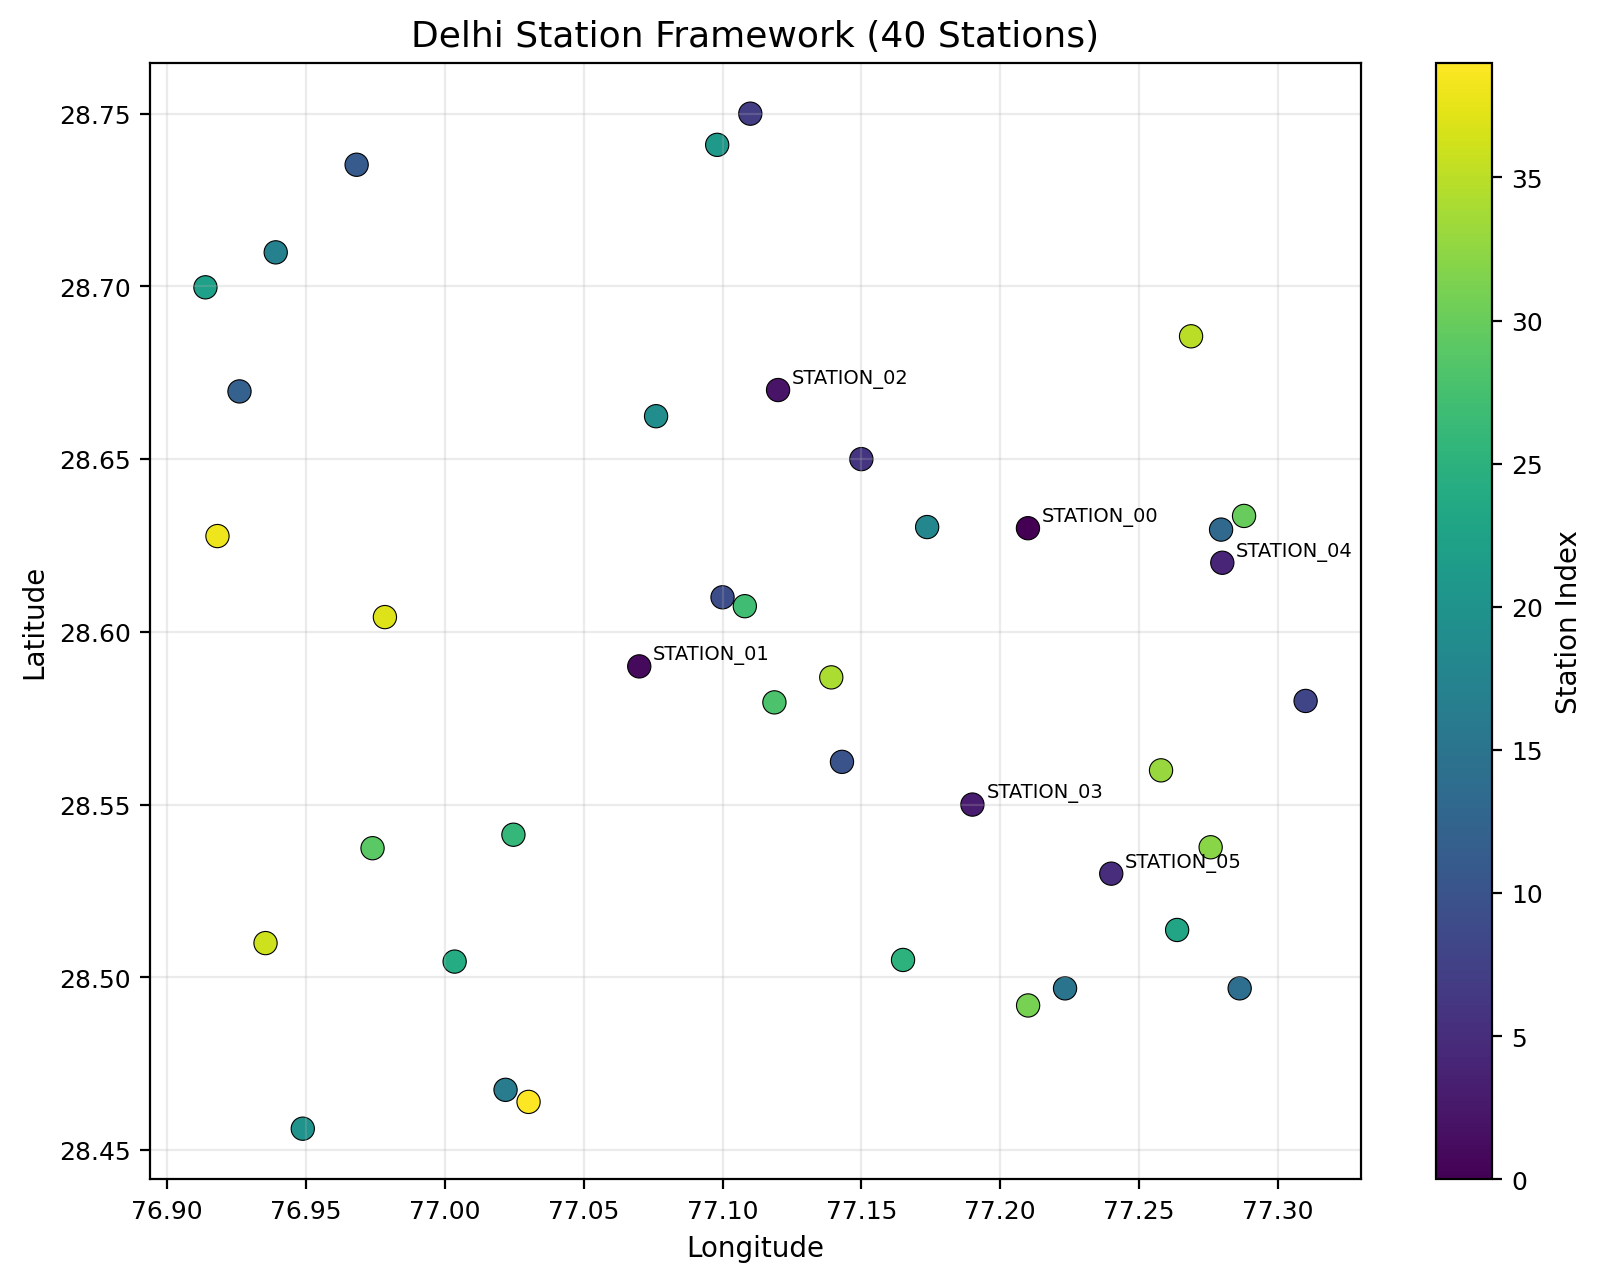
\includegraphics[width=0.86\textwidth]{images/slide07_station_coverage_map.png}
    \caption{Station coverage map}
\end{figure}

\begin{figure}[H]
    \centering
    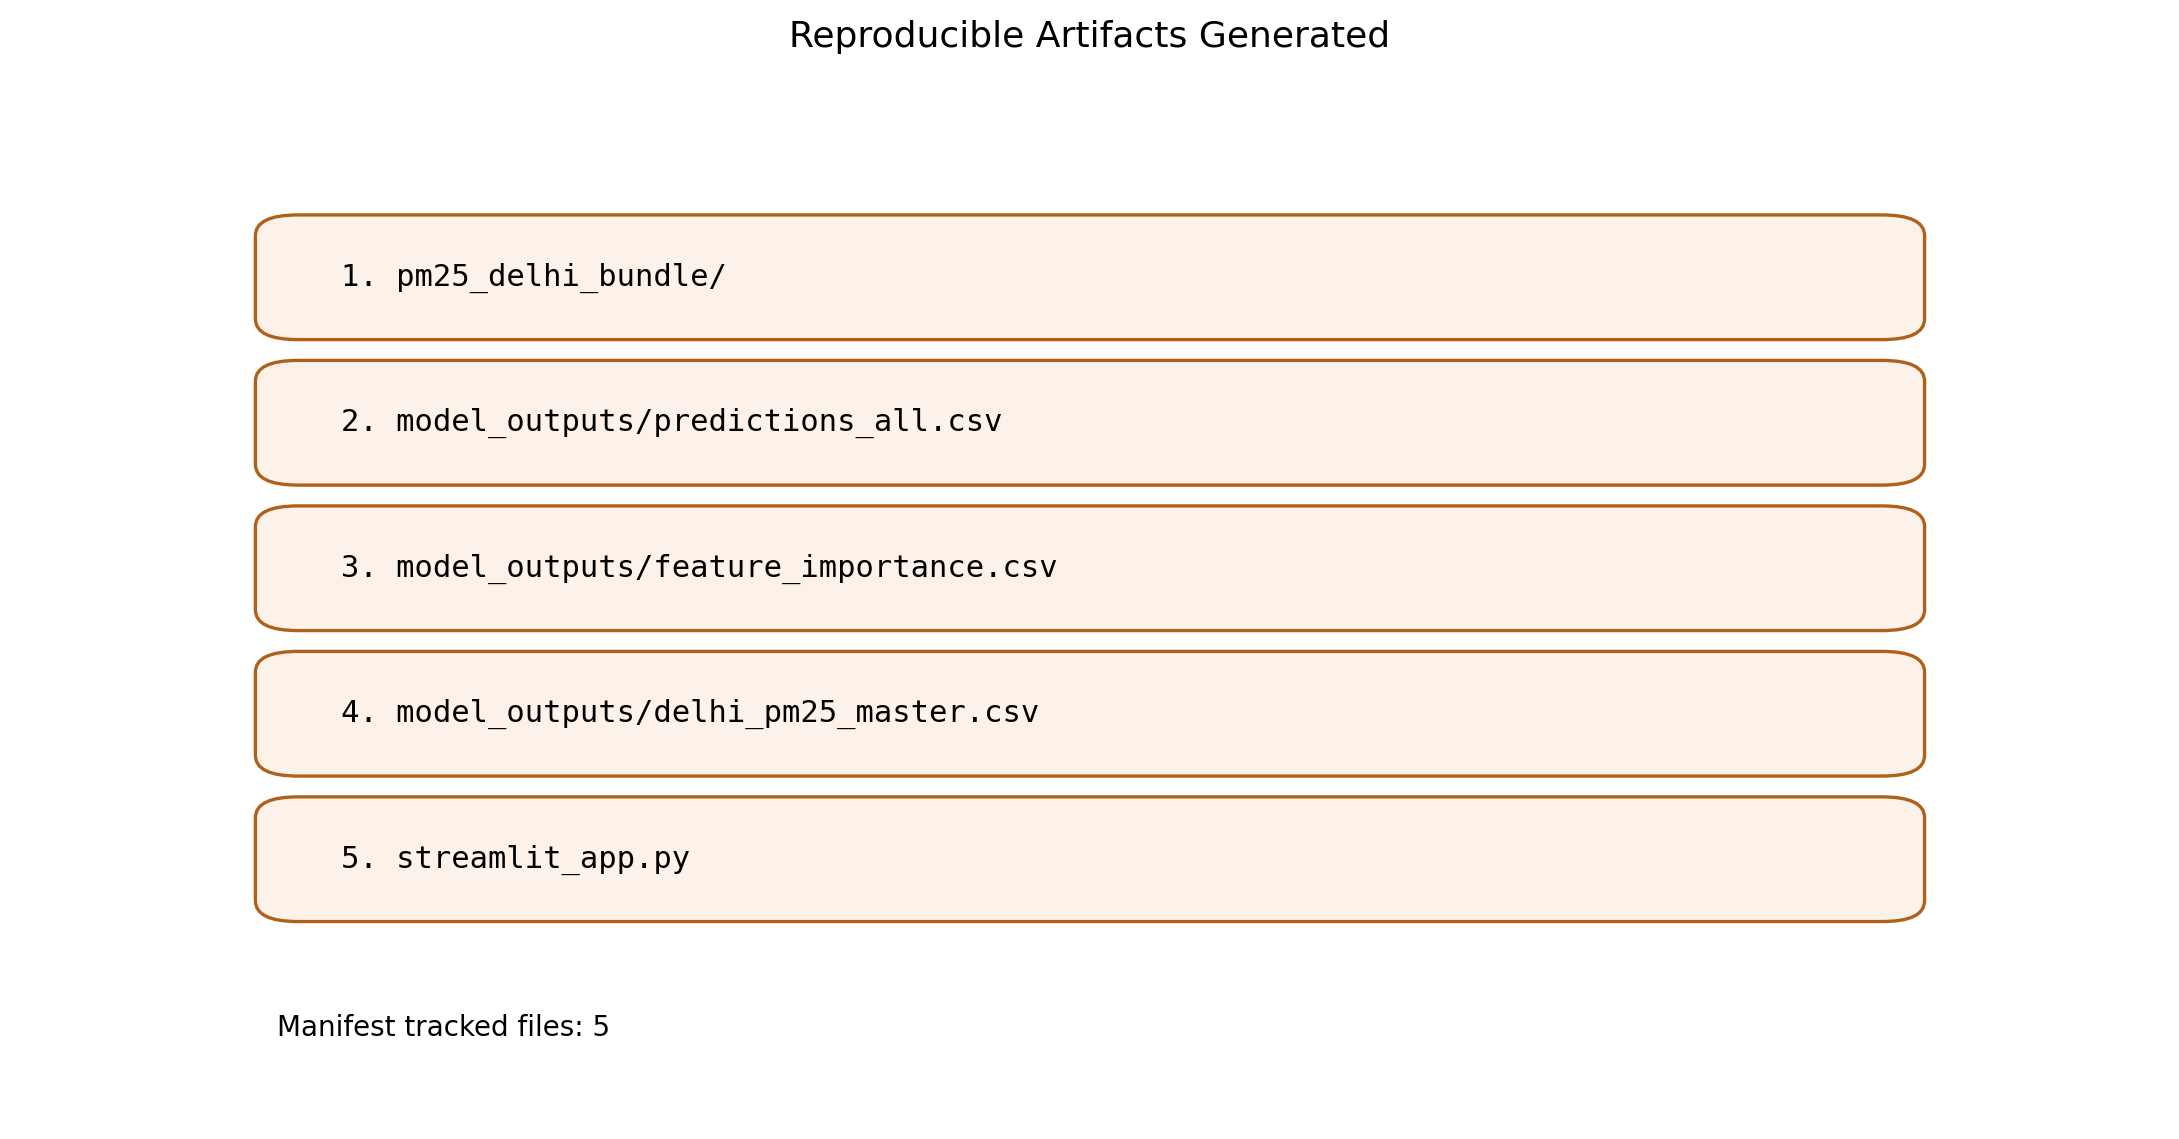
\includegraphics[width=0.82\textwidth]{images/slide14_artifacts_snapshot.png}
    \caption{Artifacts snapshot from the project outputs}
\end{figure}

\end{document}
